% CREATED BY DAVID FRISK, 2016
\chapter{Results}
\label{ch-results}
Due to computational constraints, we constrain ourselves to 7 Atari games.
Both DQN and Rainbow perform well by themselves on the chosen games.
However, the games vary in visual complexity and control problem difficulty.
In particular, the selected games are: 
\begin{enumerate}
		\item Breakout
		\item Enduro
		\item Ms Pacman
		\item Pong
		\item Qbert
		\item Seaquest
		\item Space Invaders
\end{enumerate}

Because we can only indirectly gauge the effect of various metrics through 
final algorithm performance, the primary metric of interest is obtained 
return in relation to the number of training iterations.
Due to different reward scaling, we keep results on different games in separate graphs.
We further divide the results into those pertaining to different hypotheses
in order to avoid line clutter.
As a final note, the results for each particular setting are \textbf{single-runs}.
Generally speaking, this is not adequate due to high pseudorandom number generator seed 
dependence and noisiness of reinforcement learning in general. 
Depending on the problem, 3-10 runs are averaged, or the best one is selected,
in order to tackle this problem.

\section{Effectiveness of pretrained encoders}
\label{sec-effectiveness-of-pretrained}
To begin, we first need to estimate the possible sample-efficiency gains.
This is done by comparing returns per training step between only reinforcement learning
and only reinforcement learning where training starts with a encoder
trained from the first reinforcement learning-only run.
We will use runs with reinforcement learning only as the baseline for all cases.
Because we chose games which can be essentially solved with only reinforcement learning,
the encoder of a network trained with reinforcement learning should serve
as an ideal pretrained encoder.

\begin{figure}[!t]
  \captionsetup[subfloat]{position=top,labelformat=empty}
  \centering
    \subfloat[]{  \resizebox{0.4\textwidth}{!}{
%\definecolor{blue}{RGB}{76,100,135}
%\definecolor{red}{RGB}{153,0,0}
%\definecolor{yellow}{RGB}{227,178,60}
%\definecolor{mycolor1}{rgb}{0.00000,0.44700,0.74100}%
%\definecolor{mycolor2}{rgb}{0.85000,0.32500,0.09800}%
%\definecolor{mycolor3}{rgb}{0.92900,0.69400,0.12500}%
%
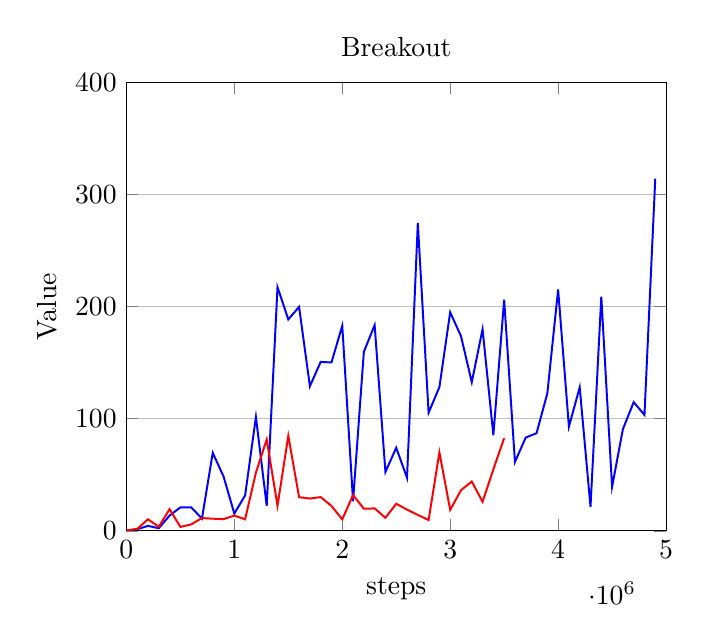
\begin{tikzpicture}

\begin{axis}[%
legend entries={rl-only-small-net,L2-reg,parallel-fs-50-no-aug}, 
legend columns=2,
title=Breakout,
legend to name=named,
legend style={legend cell align=left},
%%width=10in,
%%height=5in,
%%at={(2.596in,2.358in)},
% scale only axis,
xmin=0,
xmax=5000000,
xlabel style={font=\color{white!15!black}},
xlabel={steps},
xlabel near ticks,
ymin=0,
ymax=400,
ylabel style={font=\color{white!15!black}},
ylabel={Value},
ylabel near ticks,
ymajorgrids,
% %scale=0.5,
%%scale=0.4,
axis background/.style={fill=white},
%legend columns=2,
%legend=south outside
]
\addplot [color=blue, line width = 0.25mm]
                table[row sep=crcr]{
                  0 0.20000000298023224\\ 
100000 1.399999976158142\\ 
200000 4.400000095367432\\ 
300000 2.299999952316284\\ 
400000 13.600000381469727\\ 
500000 20.899999618530273\\ 
600000 21.0\\ 
700000 10.899999618530273\\ 
800000 69.5999984741211\\ 
900000 48.5\\ 
1000000 15.399999618530273\\ 
1100000 31.600000381469727\\ 
1200000 101.5999984741211\\ 
1300000 22.399999618530273\\ 
1400000 217.39999389648438\\ 
1500000 188.60000610351562\\ 
1600000 199.8000030517578\\ 
1700000 129.0\\ 
1800000 150.6999969482422\\ 
1900000 150.1999969482422\\ 
2000000 183.0\\ 
2100000 26.399999618530273\\ 
2200000 159.6999969482422\\ 
2300000 183.5\\ 
2400000 52.5\\ 
2500000 74.0999984741211\\ 
2600000 47.29999923706055\\ 
2700000 274.6000061035156\\ 
2800000 105.4000015258789\\ 
2900000 128.1999969482422\\ 
3000000 195.0\\ 
3100000 173.6999969482422\\ 
3200000 132.60000610351562\\ 
3300000 179.89999389648438\\ 
3400000 85.19999694824219\\ 
3500000 206.1999969482422\\ 
3600000 61.5\\ 
3700000 83.19999694824219\\ 
3800000 87.0999984741211\\ 
3900000 122.5999984741211\\ 
4000000 215.3000030517578\\ 
4100000 92.9000015258789\\ 
4200000 128.0\\ 
4300000 21.399999618530273\\ 
4400000 208.89999389648438\\ 
4500000 39.20000076293945\\ 
4600000 90.5999984741211\\ 
4700000 114.80000305175781\\ 
4800000 103.4000015258789\\ 
4900000 314.20001220703125\\ 
};
\addplot [color=red, line width = 0.25mm]
                table[row sep=crcr]{
                  0 0.4000000059604645\\ 
100000 1.7000000476837158\\ 
200000 10.300000190734863\\ 
300000 3.5999999046325684\\ 
400000 19.299999237060547\\ 
500000 3.5\\ 
600000 5.699999809265137\\ 
700000 11.399999618530273\\ 
800000 10.800000190734863\\ 
900000 10.399999618530273\\ 
1000000 13.600000381469727\\ 
1100000 10.300000190734863\\ 
1200000 51.900001525878906\\ 
1300000 81.5\\ 
1400000 22.299999237060547\\ 
1500000 84.69999694824219\\ 
1600000 30.0\\ 
1700000 28.799999237060547\\ 
1800000 30.100000381469727\\ 
1900000 22.200000762939453\\ 
2000000 10.199999809265137\\ 
2100000 31.899999618530273\\ 
2200000 19.700000762939453\\ 
2300000 20.0\\ 
2400000 11.600000381469727\\ 
2500000 24.200000762939453\\ 
2600000 18.899999618530273\\ 
2700000 14.199999809265137\\ 
2800000 9.600000381469727\\ 
2900000 70.0\\ 
3000000 18.700000762939453\\ 
3100000 36.20000076293945\\ 
3200000 44.0\\ 
3300000 25.899999618530273\\ 
3400000 54.900001525878906\\ 
3500000 82.69999694824219\\ 
};
\addplot [color=yellow, line width = 0.25mm]
                table[row sep=crcr]{
                  0 0.800000011920929\\ 
};
\end{axis}
\end{tikzpicture}}}
    \subfloat[]{  \resizebox{0.4\textwidth}{!}{
%\definecolor{blue}{RGB}{76,100,135}
%\definecolor{red}{RGB}{153,0,0}
%\definecolor{yellow}{RGB}{227,178,60}
%\definecolor{mycolor1}{rgb}{0.00000,0.44700,0.74100}%
%\definecolor{mycolor2}{rgb}{0.85000,0.32500,0.09800}%
%\definecolor{mycolor3}{rgb}{0.92900,0.69400,0.12500}%
%
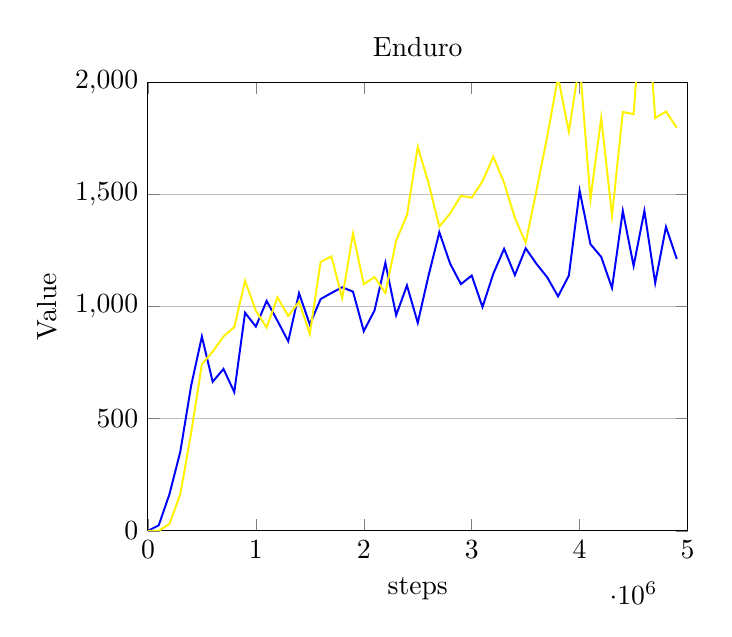
\begin{tikzpicture}

\begin{axis}[%
title=Enduro,
% %width=4.634in,
%%width=10in,
%%height=5in,
%at={(2.596in,2.358in)},
% scale only axis,
xmin=0,
xmax=5000000,
xlabel style={font=\color{white!15!black}},
xlabel={steps},
xlabel near ticks,
ymin=0,
ymax=2000,
ylabel style={font=\color{white!15!black}},
ylabel={Value},
ylabel near ticks,
ymajorgrids,
% %scale=0.5,
%scale=0.4,
axis background/.style={fill=white},
%legend style={legend cell align=left, align=left, draw=white!15!black}
]
\addplot [color=blue, line width = 0.25mm]
                table[row sep=crcr]{
                  0 0.0\\ 
100000 24.299999237060547\\ 
200000 164.3000030517578\\ 
300000 353.0\\ 
400000 646.4000244140625\\ 
500000 866.7000122070312\\ 
600000 664.7000122070312\\ 
700000 722.2000122070312\\ 
800000 618.9000244140625\\ 
900000 972.7999877929688\\ 
1000000 910.9000244140625\\ 
1100000 1025.699951171875\\ 
1200000 937.0\\ 
1300000 845.5999755859375\\ 
1400000 1059.9000244140625\\ 
1500000 920.2999877929688\\ 
1600000 1033.800048828125\\ 
1700000 1061.0\\ 
1800000 1086.5999755859375\\ 
1900000 1066.9000244140625\\ 
2000000 890.9000244140625\\ 
2100000 983.5\\ 
2200000 1195.300048828125\\ 
2300000 962.0\\ 
2400000 1094.800048828125\\ 
2500000 928.0\\ 
2600000 1138.5999755859375\\ 
2700000 1332.300048828125\\ 
2800000 1191.800048828125\\ 
2900000 1100.5999755859375\\ 
3000000 1138.800048828125\\ 
3100000 998.2999877929688\\ 
3200000 1146.800048828125\\ 
3300000 1258.0999755859375\\ 
3400000 1141.0\\ 
3500000 1260.300048828125\\ 
3600000 1190.800048828125\\ 
3700000 1130.5999755859375\\ 
3800000 1046.0999755859375\\ 
3900000 1138.4000244140625\\ 
4000000 1517.5\\ 
4100000 1278.9000244140625\\ 
4200000 1221.699951171875\\ 
4300000 1083.199951171875\\ 
4400000 1426.9000244140625\\ 
4500000 1181.5999755859375\\ 
4600000 1427.199951171875\\ 
4700000 1105.800048828125\\ 
4800000 1355.800048828125\\ 
4900000 1212.9000244140625\\ 
};
\addplot [color=red, line width = 0.25mm]
                table[row sep=crcr]{
                  0 0.0\\ 
};
\addplot [color=yellow, line width = 0.25mm]
                table[row sep=crcr]{
                  0 0.0\\ 
100000 0.0\\ 
200000 30.700000762939453\\ 
300000 163.6999969482422\\ 
400000 435.79998779296875\\ 
500000 743.2000122070312\\ 
600000 799.2000122070312\\ 
700000 867.0\\ 
800000 908.4000244140625\\ 
900000 1115.300048828125\\ 
1000000 981.4000244140625\\ 
1100000 906.9000244140625\\ 
1200000 1041.5999755859375\\ 
1300000 958.5999755859375\\ 
1400000 1021.9000244140625\\ 
1500000 877.7000122070312\\ 
1600000 1199.4000244140625\\ 
1700000 1224.0\\ 
1800000 1038.199951171875\\ 
1900000 1326.0999755859375\\ 
2000000 1100.0\\ 
2100000 1132.0999755859375\\ 
2200000 1060.9000244140625\\ 
2300000 1294.300048828125\\ 
2400000 1407.699951171875\\ 
2500000 1712.5\\ 
2600000 1551.5\\ 
2700000 1357.0\\ 
2800000 1415.800048828125\\ 
2900000 1494.5\\ 
3000000 1486.0\\ 
3100000 1559.699951171875\\ 
3200000 1668.5\\ 
3300000 1552.800048828125\\ 
3400000 1395.800048828125\\ 
3500000 1284.9000244140625\\ 
3600000 1518.0\\ 
3700000 1759.5999755859375\\ 
3800000 2024.9000244140625\\ 
3900000 1780.0999755859375\\ 
4000000 2090.5\\ 
4100000 1479.0999755859375\\ 
4200000 1841.699951171875\\ 
4300000 1405.5999755859375\\ 
4400000 1868.300048828125\\ 
4500000 1858.699951171875\\ 
4600000 2527.0\\ 
4700000 1841.0\\ 
4800000 1870.800048828125\\ 
4900000 1797.9000244140625\\ 
};
\end{axis}
\end{tikzpicture}}}\\
  \vspace{-1cm}
    \subfloat[]{  \resizebox{0.4\textwidth}{!}{
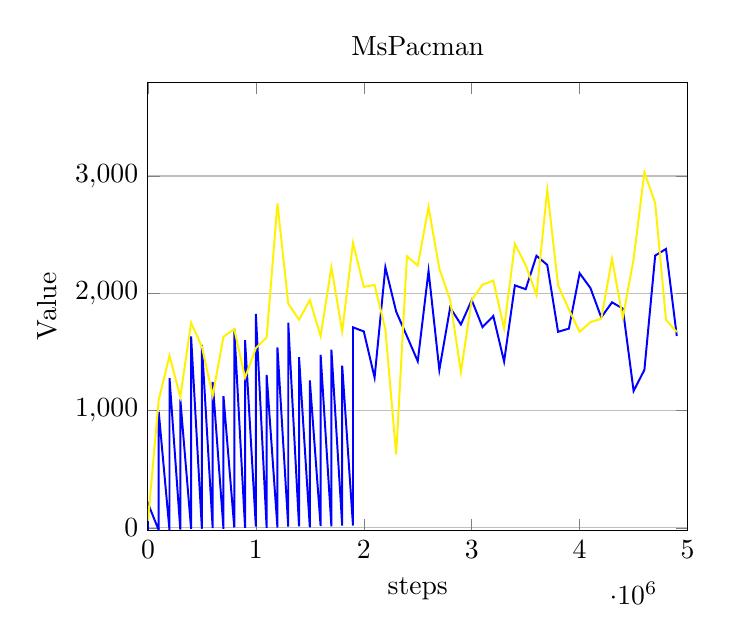
\begin{tikzpicture}

\begin{axis}[%
title=MsPacman,
% %width=4.634in,
%width=10in,
%height=5in,
%at={(2.596in,2.358in)},
% scale only axis,
xmin=0,
xmax=5000000,
xlabel style={font=\color{white!15!black}},
xlabel={steps},
xlabel near ticks,
ymin=-22,
ymax=3800,
ylabel style={font=\color{white!15!black}},
ylabel={Value},
ylabel near ticks,
ymajorgrids,
% %scale=0.5,
%scale=0.4,
axis background/.style={fill=white},
%legend style={legend cell align=left, align=left, draw=white!15!black}
]
\addplot [color=blue, line width = 0.25mm]
                table[row sep=crcr]{
                  0 -21.0\\ 
0 210.0\\ 
100000 -19.799999237060547\\ 
100000 990.0\\ 
200000 -20.700000762939453\\ 
200000 1277.0\\ 
300000 -15.0\\ 
300000 1096.0\\ 
400000 -7.0\\ 
400000 1632.0\\ 
500000 -6.900000095367432\\ 
500000 1561.0\\ 
600000 -1.899999976158142\\ 
600000 1245.0\\ 
700000 -7.599999904632568\\ 
700000 1123.0\\ 
800000 4.0\\ 
800000 1696.0\\ 
900000 1.5\\ 
900000 1600.0\\ 
1000000 11.300000190734863\\ 
1000000 1824.0\\ 
1100000 1.2000000476837158\\ 
1100000 1304.0\\ 
1200000 3.700000047683716\\ 
1200000 1538.0\\ 
1300000 11.5\\ 
1300000 1750.0\\ 
1400000 13.600000381469727\\ 
1400000 1456.0\\ 
1500000 5.699999809265137\\ 
1500000 1258.0\\ 
1600000 15.600000381469727\\ 
1600000 1476.0\\ 
1700000 13.5\\ 
1700000 1519.0\\ 
1800000 19.299999237060547\\ 
1800000 1383.0\\ 
1900000 20.799999237060547\\ 
1900000 1710.0\\ 
2000000 1675.0\\ 
2100000 1282.0\\ 
2200000 2222.0\\ 
2300000 1844.0\\ 
2400000 1634.0\\ 
2500000 1421.0\\ 
2600000 2191.0\\ 
2700000 1347.0\\ 
2800000 1878.0\\ 
2900000 1735.0\\ 
3000000 1942.0\\ 
3100000 1712.0\\ 
3200000 1806.0\\ 
3300000 1419.0\\ 
3400000 2068.0\\ 
3500000 2035.0\\ 
3600000 2320.0\\ 
3700000 2242.0\\ 
3800000 1672.0\\ 
3900000 1699.0\\ 
4000000 2171.0\\ 
4100000 2045.0\\ 
4200000 1795.0\\ 
4300000 1923.0\\ 
4400000 1870.0\\ 
4500000 1167.0\\ 
4600000 1348.0\\ 
4700000 2322.0\\ 
4800000 2378.0\\ 
4900000 1636.0\\ 
};
\addplot [color=red, line width = 0.25mm]
                table[row sep=crcr]{
                  0 0.0\\ 
};
\addplot [color=yellow, line width = 0.25mm]
                table[row sep=crcr]{
                  0 60.0\\ 
100000 1090.0\\ 
200000 1469.0\\ 
300000 1117.0\\ 
400000 1749.0\\ 
500000 1545.0\\ 
600000 1128.0\\ 
700000 1630.0\\ 
800000 1695.0\\ 
900000 1281.0\\ 
1000000 1532.0\\ 
1100000 1625.0\\ 
1200000 2767.0\\ 
1300000 1912.0\\ 
1400000 1775.0\\ 
1500000 1942.0\\ 
1600000 1636.0\\ 
1700000 2222.0\\ 
1800000 1676.0\\ 
1900000 2430.0\\ 
2000000 2055.0\\ 
2100000 2072.0\\ 
2200000 1693.0\\ 
2300000 625.0\\ 
2400000 2317.0\\ 
2500000 2236.0\\ 
2600000 2736.0\\ 
2700000 2209.0\\ 
2800000 1944.0\\ 
2900000 1329.0\\ 
3000000 1944.0\\ 
3100000 2074.0\\ 
3200000 2109.0\\ 
3300000 1701.0\\ 
3400000 2421.0\\ 
3500000 2240.0\\ 
3600000 1986.0\\ 
3700000 2883.0\\ 
3800000 2069.0\\ 
3900000 1863.0\\ 
4000000 1672.0\\ 
4100000 1754.0\\ 
4200000 1783.0\\ 
4300000 2293.0\\ 
4400000 1791.0\\ 
4500000 2293.0\\ 
4600000 3033.0\\ 
4700000 2768.0\\ 
4800000 1774.0\\ 
4900000 1670.0\\ 
};
\end{axis}
\end{tikzpicture}}}
    \subfloat[]{  \resizebox{0.4\textwidth}{!}{
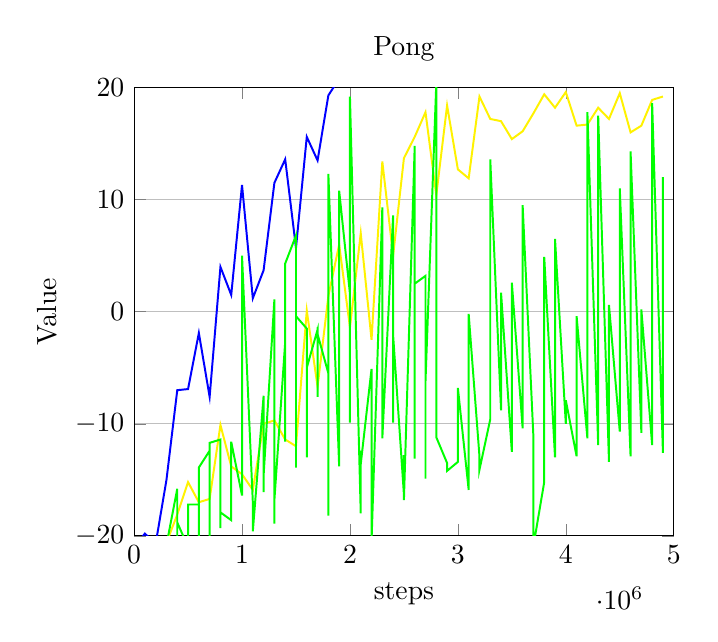
\begin{tikzpicture}

\begin{axis}[%
title=Pong,
% %width=4.634in,
%width=10in,
%height=5in,
%at={(2.596in,2.358in)},
% scale only axis,
xmin=0,
xmax=5000000,
xlabel style={font=\color{white!15!black}},
xlabel={steps},
xlabel near ticks,
ymin=-20,
ymax=20,
ylabel style={font=\color{white!15!black}},
ylabel={Value},
ylabel near ticks,
ymajorgrids,
% %scale=0.5,
%scale=0.4,
axis background/.style={fill=white},
%legend style={legend cell align=left, align=left, draw=white!15!black}
]
\addplot [color=blue, line width = 0.25mm]
                table[row sep=crcr]{
                  0 -21.0\\ 
100000 -19.799999237060547\\ 
200000 -20.700000762939453\\ 
300000 -15.0\\ 
400000 -7.0\\ 
500000 -6.900000095367432\\ 
600000 -1.899999976158142\\ 
700000 -7.599999904632568\\ 
800000 4.0\\ 
900000 1.5\\ 
1000000 11.300000190734863\\ 
1100000 1.2000000476837158\\ 
1200000 3.700000047683716\\ 
1300000 11.5\\ 
1400000 13.600000381469727\\ 
1500000 5.699999809265137\\ 
1600000 15.600000381469727\\ 
1700000 13.5\\ 
1800000 19.299999237060547\\ 
1900000 20.799999237060547\\ 
};
\addplot [color=red, line width = 0.25mm]
                table[row sep=crcr]{
                  0 0.0\\ 
};
\addplot [color=yellow, line width = 0.25mm]
                table[row sep=crcr]{
                  0 -21.0\\ 
0 -21.0\\ 
0 -21.0\\ 
100000 -21.0\\ 
200000 -20.299999237060547\\ 
300000 -20.600000381469727\\ 
400000 -18.100000381469727\\ 
500000 -15.199999809265137\\ 
600000 -17.0\\ 
700000 -16.700000762939453\\ 
800000 -10.100000381469727\\ 
900000 -13.800000190734863\\ 
1000000 -14.5\\ 
1100000 -15.899999618530273\\ 
1200000 -10.0\\ 
1300000 -9.699999809265137\\ 
1400000 -11.399999618530273\\ 
1500000 -12.0\\ 
1600000 0.10000000149011612\\ 
1700000 -6.699999809265137\\ 
1800000 1.399999976158142\\ 
1900000 6.0\\ 
2000000 -1.399999976158142\\ 
2100000 7.0\\ 
2200000 -2.5\\ 
2300000 13.399999618530273\\ 
2400000 5.0\\ 
2500000 13.699999809265137\\ 
2600000 15.600000381469727\\ 
2700000 17.799999237060547\\ 
2800000 10.399999618530273\\ 
2900000 18.399999618530273\\ 
3000000 12.699999809265137\\ 
3100000 11.899999618530273\\ 
3200000 19.200000762939453\\ 
3300000 17.200000762939453\\ 
3400000 17.0\\ 
3500000 15.399999618530273\\ 
3600000 16.100000381469727\\ 
3700000 17.700000762939453\\ 
3800000 19.399999618530273\\ 
3900000 18.200000762939453\\ 
4000000 19.600000381469727\\ 
4100000 16.600000381469727\\ 
4200000 16.700000762939453\\ 
4300000 18.200000762939453\\ 
4400000 17.200000762939453\\ 
4500000 19.5\\ 
4600000 16.0\\ 
4700000 16.600000381469727\\ 
4800000 18.899999618530273\\ 
4900000 19.200000762939453\\ 
};
\addplot [color=green, line width = 0.25mm]
                table[row sep=crcr]{
                  0 -21.0\\ 
0 -21.0\\ 
0 -21.0\\ 
0 -21.0\\ 
100000 -21.0\\ 
100000 -20.600000381469727\\ 
100000 -21.0\\ 
200000 -20.399999618530273\\ 
200000 -21.0\\ 
200000 -20.799999237060547\\ 
300000 -20.600000381469727\\ 
300000 -20.799999237060547\\ 
300000 -20.799999237060547\\ 
400000 -15.800000190734863\\ 
400000 -20.399999618530273\\ 
400000 -18.799999237060547\\ 
500000 -21.0\\ 
500000 -21.0\\ 
500000 -17.200000762939453\\ 
600000 -17.200000762939453\\ 
600000 -20.600000381469727\\ 
600000 -13.899999618530273\\ 
700000 -12.399999618530273\\ 
700000 -20.100000381469727\\ 
700000 -11.699999809265137\\ 
800000 -11.399999618530273\\ 
800000 -19.299999237060547\\ 
800000 -17.899999618530273\\ 
900000 -18.600000381469727\\ 
900000 -15.699999809265137\\ 
900000 -11.600000381469727\\ 
1000000 -16.399999618530273\\ 
1000000 -16.0\\ 
1000000 5.0\\ 
1100000 -17.0\\ 
1100000 -17.5\\ 
1100000 -19.600000381469727\\ 
1200000 -7.5\\ 
1200000 -16.100000381469727\\ 
1200000 -14.600000381469727\\ 
1300000 1.100000023841858\\ 
1300000 -18.899999618530273\\ 
1300000 -16.799999237060547\\ 
1400000 -2.700000047683716\\ 
1400000 -11.600000381469727\\ 
1400000 4.300000190734863\\ 
1500000 6.800000190734863\\ 
1500000 -13.899999618530273\\ 
1500000 -0.4000000059604645\\ 
1600000 -1.5\\ 
1600000 -13.0\\ 
1600000 -5.0\\ 
1700000 -1.600000023841858\\ 
1700000 -7.599999904632568\\ 
1700000 -2.0\\ 
1800000 -5.5\\ 
1800000 -18.200000762939453\\ 
1800000 12.300000190734863\\ 
1900000 -13.800000190734863\\ 
1900000 -10.0\\ 
1900000 10.800000190734863\\ 
2000000 1.600000023841858\\ 
2000000 -9.899999618530273\\ 
2000000 19.200000762939453\\ 
2100000 -18.0\\ 
2100000 -12.399999618530273\\ 
2100000 -13.600000381469727\\ 
2200000 -5.099999904632568\\ 
2200000 -13.899999618530273\\ 
2200000 -20.5\\ 
2300000 9.300000190734863\\ 
2300000 -8.199999809265137\\ 
2300000 -11.300000190734863\\ 
2400000 8.600000381469727\\ 
2400000 -9.899999618530273\\ 
2400000 -2.0999999046325684\\ 
2500000 -16.299999237060547\\ 
2500000 -12.800000190734863\\ 
2500000 -16.799999237060547\\ 
2600000 14.800000190734863\\ 
2600000 -13.100000381469727\\ 
2600000 2.5\\ 
2700000 3.200000047683716\\ 
2700000 -14.899999618530273\\ 
2700000 -6.199999809265137\\ 
2800000 20.399999618530273\\ 
2800000 -9.800000190734863\\ 
2800000 -11.199999809265137\\ 
2900000 -13.5\\ 
2900000 -14.199999809265137\\ 
3000000 -13.399999618530273\\ 
3000000 -6.800000190734863\\ 
3100000 -15.899999618530273\\ 
3100000 -0.20000000298023224\\ 
3200000 -12.899999618530273\\ 
3200000 -14.100000381469727\\ 
3300000 -9.600000381469727\\ 
3300000 13.600000381469727\\ 
3400000 -8.800000190734863\\ 
3400000 1.7000000476837158\\ 
3500000 -12.5\\ 
3500000 2.5999999046325684\\ 
3600000 -10.399999618530273\\ 
3600000 9.5\\ 
3700000 -11.199999809265137\\ 
3700000 -20.899999618530273\\ 
3800000 -15.199999809265137\\ 
3800000 4.900000095367432\\ 
3900000 -13.0\\ 
3900000 6.5\\ 
4000000 -10.0\\ 
4000000 -7.900000095367432\\ 
4100000 -12.899999618530273\\ 
4100000 -0.4000000059604645\\ 
4200000 -11.300000190734863\\ 
4200000 17.799999237060547\\ 
4300000 -11.899999618530273\\ 
4300000 17.5\\ 
4400000 -13.399999618530273\\ 
4400000 0.6000000238418579\\ 
4500000 -10.699999809265137\\ 
4500000 11.0\\ 
4600000 -12.899999618530273\\ 
4600000 14.300000190734863\\ 
4700000 -10.800000190734863\\ 
4700000 0.20000000298023224\\ 
4800000 -11.899999618530273\\ 
4800000 18.600000381469727\\ 
4900000 -12.600000381469727\\ 
4900000 12.0\\ 
};
\end{axis}
\end{tikzpicture}}}\\
  \vspace{-1cm}
    \subfloat[]{  \resizebox{0.4\textwidth}{!}{
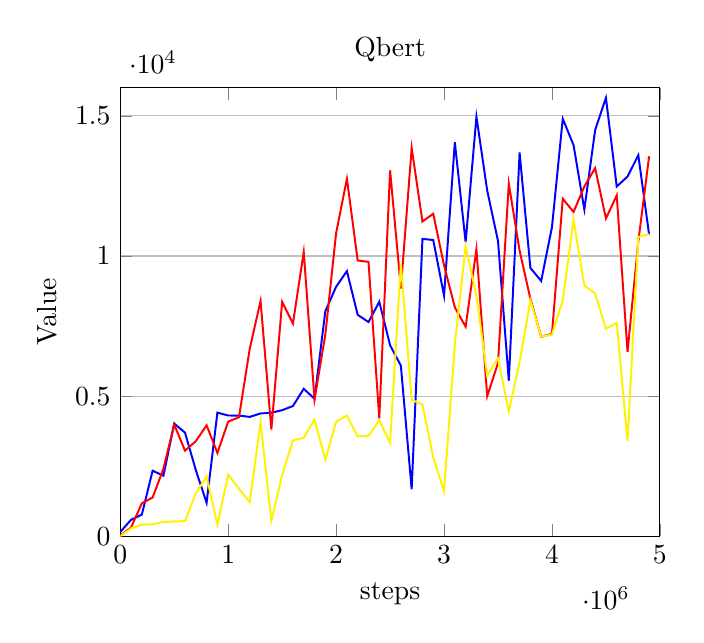
\begin{tikzpicture}

\begin{axis}[%
title=Qbert,
% %width=4.634in,
%width=10in,
%height=5in,
%at={(2.596in,2.358in)},
% scale only axis,
xmin=0,
xmax=5000000,
xlabel style={font=\color{white!15!black}},
xlabel={steps},
xlabel near ticks,
ymin=0,
ymax=16000,
ylabel style={font=\color{white!15!black}},
ylabel={Value},
ylabel near ticks,
ymajorgrids,
% %scale=0.5,
%scale=0.4,
axis background/.style={fill=white},
%legend style={legend cell align=left, align=left, draw=white!15!black}
]
\addplot [color=blue, line width = 0.25mm]
                table[row sep=crcr]{
                  0 150.0\\ 
100000 585.0\\ 
200000 772.5\\ 
300000 2337.5\\ 
400000 2157.5\\ 
500000 4022.5\\ 
600000 3695.0\\ 
700000 2362.5\\ 
800000 1192.5\\ 
900000 4410.0\\ 
1000000 4307.5\\ 
1100000 4305.0\\ 
1200000 4257.5\\ 
1300000 4380.0\\ 
1400000 4407.5\\ 
1500000 4497.5\\ 
1600000 4645.0\\ 
1700000 5260.0\\ 
1800000 4905.0\\ 
1900000 8030.0\\ 
2000000 8902.5\\ 
2100000 9460.0\\ 
2200000 7900.0\\ 
2300000 7642.5\\ 
2400000 8367.5\\ 
2500000 6815.0\\ 
2600000 6085.0\\ 
2700000 1677.5\\ 
2800000 10610.0\\ 
2900000 10570.0\\ 
3000000 8585.0\\ 
3100000 14057.5\\ 
3200000 10490.0\\ 
3300000 14970.0\\ 
3400000 12332.5\\ 
3500000 10537.5\\ 
3600000 5550.0\\ 
3700000 13692.5\\ 
3800000 9572.5\\ 
3900000 9110.0\\ 
4000000 11030.0\\ 
4100000 14897.5\\ 
4200000 13955.0\\ 
4300000 11660.0\\ 
4400000 14495.0\\ 
4500000 15645.0\\ 
4600000 12480.0\\ 
4700000 12835.0\\ 
4800000 13597.5\\ 
4900000 10762.5\\ 
};
\addplot [color=red, line width = 0.25mm]
                table[row sep=crcr]{
                  0 22.5\\ 
100000 310.0\\ 
200000 1172.5\\ 
300000 1382.5\\ 
400000 2410.0\\ 
500000 3982.5\\ 
600000 3052.5\\ 
700000 3390.0\\ 
800000 3957.5\\ 
900000 2970.0\\ 
1000000 4090.0\\ 
1100000 4245.0\\ 
1200000 6697.5\\ 
1300000 8395.0\\ 
1400000 3807.5\\ 
1500000 8360.0\\ 
1600000 7590.0\\ 
1700000 10142.5\\ 
1800000 4877.5\\ 
1900000 7190.0\\ 
2000000 10817.5\\ 
2100000 12755.0\\ 
2200000 9840.0\\ 
2300000 9790.0\\ 
2400000 4202.5\\ 
2500000 13057.5\\ 
2600000 8842.5\\ 
2700000 13852.5\\ 
2800000 11230.0\\ 
2900000 11507.5\\ 
3000000 9665.0\\ 
3100000 8167.5\\ 
3200000 7475.0\\ 
3300000 10242.5\\ 
3400000 4997.5\\ 
3500000 6180.0\\ 
3600000 12582.5\\ 
3700000 10190.0\\ 
3800000 8475.0\\ 
3900000 7115.0\\ 
4000000 7222.5\\ 
4100000 12042.5\\ 
4200000 11572.5\\ 
4300000 12480.0\\ 
4400000 13137.5\\ 
4500000 11337.5\\ 
4600000 12165.0\\ 
4700000 6580.0\\ 
4800000 10517.5\\ 
4900000 13560.0\\ 
};
\addplot [color=yellow, line width = 0.25mm]
                table[row sep=crcr]{
                  0 0.0\\ 
100000 280.0\\ 
200000 415.0\\ 
300000 425.0\\ 
400000 507.5\\ 
500000 525.0\\ 
600000 537.5\\ 
700000 1525.0\\ 
800000 2137.5\\ 
900000 407.5\\ 
1000000 2195.0\\ 
1100000 1690.0\\ 
1200000 1215.0\\ 
1300000 4077.5\\ 
1400000 550.0\\ 
1500000 2185.0\\ 
1600000 3417.5\\ 
1700000 3512.5\\ 
1800000 4165.0\\ 
1900000 2730.0\\ 
2000000 4090.0\\ 
2100000 4305.0\\ 
2200000 3557.5\\ 
2300000 3585.0\\ 
2400000 4137.5\\ 
2500000 3335.0\\ 
2600000 9722.5\\ 
2700000 4865.0\\ 
2800000 4700.0\\ 
2900000 2812.5\\ 
3000000 1605.0\\ 
3100000 6847.5\\ 
3200000 10342.5\\ 
3300000 8590.0\\ 
3400000 5732.5\\ 
3500000 6345.0\\ 
3600000 4447.5\\ 
3700000 6217.5\\ 
3800000 8415.0\\ 
3900000 7120.0\\ 
4000000 7195.0\\ 
4100000 8415.0\\ 
4200000 11307.5\\ 
4300000 8942.5\\ 
4400000 8662.5\\ 
4500000 7402.5\\ 
4600000 7612.5\\ 
4700000 3395.0\\ 
4800000 10680.0\\ 
4900000 10780.0\\ 
};
\end{axis}
\end{tikzpicture}}}
    \subfloat[]{  \resizebox{0.4\textwidth}{!}{
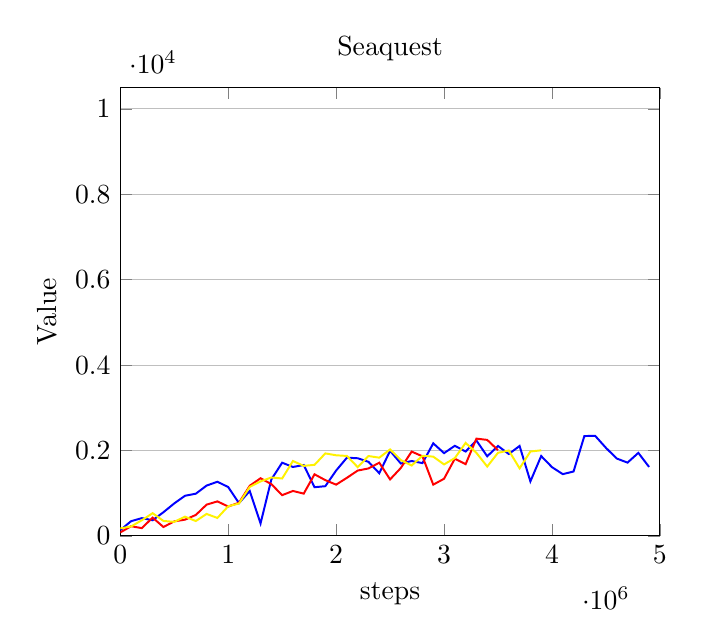
\begin{tikzpicture}

\begin{axis}[%
title=Seaquest,
% %width=4.634in,
%width=10in,
%height=5in,
%at={(2.596in,2.358in)},
% scale only axis,
xmin=0,
xmax=5000000,
xlabel style={font=\color{white!15!black}},
xlabel={steps},
xlabel near ticks,
ymin=0,
ymax=10500,
ylabel style={font=\color{white!15!black}},
ylabel={Value},
ylabel near ticks,
ymajorgrids,
% %scale=0.5,
%scale=0.4,
axis background/.style={fill=white},
%legend style={legend cell align=left, align=left, draw=white!15!black}
]
\addplot [color=blue, line width = 0.25mm]
                table[row sep=crcr]{
                  0 134.0\\ 
100000 344.0\\ 
200000 416.0\\ 
300000 366.0\\ 
400000 554.0\\ 
500000 760.0\\ 
600000 940.0\\ 
700000 988.0\\ 
800000 1178.0\\ 
900000 1268.0\\ 
1000000 1144.0\\ 
1100000 768.0\\ 
1200000 1052.0\\ 
1300000 292.0\\ 
1400000 1322.0\\ 
1500000 1714.0\\ 
1600000 1614.0\\ 
1700000 1660.0\\ 
1800000 1140.0\\ 
1900000 1164.0\\ 
2000000 1530.0\\ 
2100000 1832.0\\ 
2200000 1818.0\\ 
2300000 1734.0\\ 
2400000 1468.0\\ 
2500000 1992.0\\ 
2600000 1694.0\\ 
2700000 1754.0\\ 
2800000 1704.0\\ 
2900000 2168.0\\ 
3000000 1938.0\\ 
3100000 2110.0\\ 
3200000 1976.0\\ 
3300000 2234.0\\ 
3400000 1864.0\\ 
3500000 2106.0\\ 
3600000 1918.0\\ 
3700000 2106.0\\ 
3800000 1276.0\\ 
3900000 1870.0\\ 
4000000 1610.0\\ 
4100000 1446.0\\ 
4200000 1508.0\\ 
4300000 2338.0\\ 
4400000 2344.0\\ 
4500000 2062.0\\ 
4600000 1812.0\\ 
4700000 1716.0\\ 
4800000 1944.0\\ 
4900000 1614.0\\ 
};
\addplot [color=red, line width = 0.25mm]
                table[row sep=crcr]{
                  0 80.0\\ 
100000 226.0\\ 
200000 182.0\\ 
300000 428.0\\ 
400000 208.0\\ 
500000 340.0\\ 
600000 380.0\\ 
700000 490.0\\ 
800000 732.0\\ 
900000 808.0\\ 
1000000 688.0\\ 
1100000 776.0\\ 
1200000 1174.0\\ 
1300000 1350.0\\ 
1400000 1212.0\\ 
1500000 954.0\\ 
1600000 1052.0\\ 
1700000 990.0\\ 
1800000 1442.0\\ 
1900000 1306.0\\ 
2000000 1200.0\\ 
2100000 1360.0\\ 
2200000 1530.0\\ 
2300000 1580.0\\ 
2400000 1714.0\\ 
2500000 1322.0\\ 
2600000 1592.0\\ 
2700000 1974.0\\ 
2800000 1864.0\\ 
2900000 1200.0\\ 
3000000 1338.0\\ 
3100000 1808.0\\ 
3200000 1680.0\\ 
3300000 2278.0\\ 
3400000 2248.0\\ 
3500000 2008.0\\ 
};
\addplot [color=yellow, line width = 0.25mm]
                table[row sep=crcr]{
                  0 176.0\\ 
100000 220.0\\ 
200000 366.0\\ 
300000 532.0\\ 
400000 350.0\\ 
500000 328.0\\ 
600000 450.0\\ 
700000 348.0\\ 
800000 514.0\\ 
900000 420.0\\ 
1000000 694.0\\ 
1100000 758.0\\ 
1200000 1148.0\\ 
1300000 1276.0\\ 
1400000 1368.0\\ 
1500000 1344.0\\ 
1600000 1754.0\\ 
1700000 1640.0\\ 
1800000 1664.0\\ 
1900000 1932.0\\ 
2000000 1888.0\\ 
2100000 1872.0\\ 
2200000 1610.0\\ 
2300000 1870.0\\ 
2400000 1832.0\\ 
2500000 2024.0\\ 
2600000 1774.0\\ 
2700000 1648.0\\ 
2800000 1876.0\\ 
2900000 1856.0\\ 
3000000 1674.0\\ 
3100000 1822.0\\ 
3200000 2178.0\\ 
3300000 1944.0\\ 
3400000 1624.0\\ 
3500000 1946.0\\ 
3600000 2000.0\\ 
3700000 1582.0\\ 
3800000 1976.0\\ 
3900000 2004.0\\ 
};
\end{axis}
\end{tikzpicture}}}\\
  \vspace{-1cm}
    \subfloat[]{  \resizebox{0.4\textwidth}{!}{
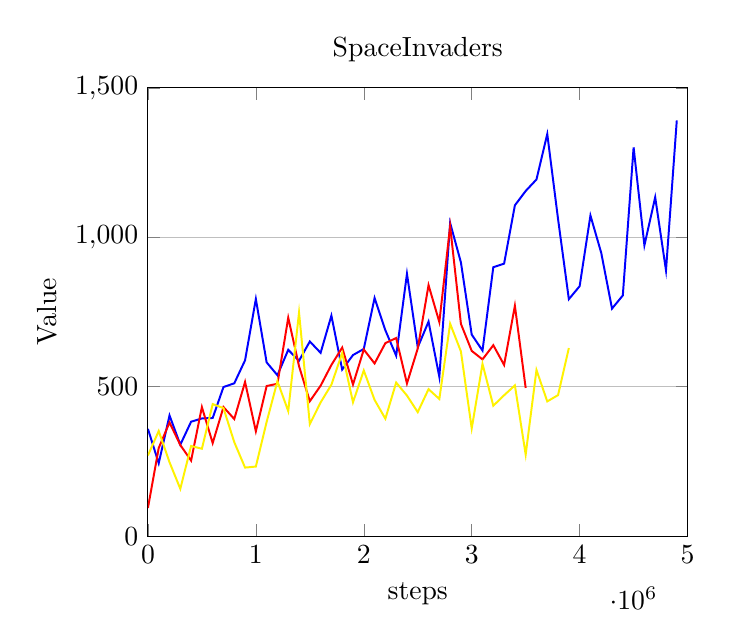
\begin{tikzpicture}

\begin{axis}[%
title=SpaceInvaders,
%width=10in,
%height=5in,
%at={(2.596in,2.358in)},
% scale only axis,
xmin=0,
xmax=5000000,
xlabel style={font=\color{white!15!black}},
xlabel={steps},
xlabel near ticks,
ymin=0,
ymax=1500,
ylabel style={font=\color{white!15!black}},
ylabel={Value},
ylabel near ticks,
ymajorgrids,
% %scale=0.5,
%scale=0.4,
axis background/.style={fill=white},
%legend style={legend cell align=left, align=left, draw=white!15!black}
]
\addplot [color=blue, line width = 0.25mm]
                table[row sep=crcr]{
                  0 359.0\\ 
100000 244.0\\ 
200000 404.0\\ 
300000 306.0\\ 
400000 383.0\\ 
500000 394.0\\ 
600000 395.5\\ 
700000 499.0\\ 
800000 511.5\\ 
900000 588.5\\ 
1000000 793.5\\ 
1100000 581.5\\ 
1200000 538.5\\ 
1300000 623.5\\ 
1400000 587.0\\ 
1500000 651.5\\ 
1600000 613.5\\ 
1700000 738.0\\ 
1800000 557.5\\ 
1900000 606.0\\ 
2000000 626.5\\ 
2100000 797.0\\ 
2200000 689.0\\ 
2300000 604.0\\ 
2400000 878.0\\ 
2500000 632.0\\ 
2600000 718.0\\ 
2700000 533.0\\ 
2800000 1048.0\\ 
2900000 916.0\\ 
3000000 674.5\\ 
3100000 621.0\\ 
3200000 900.0\\ 
3300000 912.0\\ 
3400000 1107.0\\ 
3500000 1155.0\\ 
3600000 1193.5\\ 
3700000 1345.5\\ 
3800000 1061.0\\ 
3900000 793.0\\ 
4000000 836.5\\ 
4100000 1073.0\\ 
4200000 948.0\\ 
4300000 761.5\\ 
4400000 805.5\\ 
4500000 1301.0\\ 
4600000 973.0\\ 
4700000 1134.0\\ 
4800000 889.5\\ 
4900000 1391.0\\ 
};
\addplot [color=red, line width = 0.25mm]
                table[row sep=crcr]{
                  0 94.5\\ 
100000 295.0\\ 
200000 380.5\\ 
300000 305.0\\ 
400000 253.0\\ 
500000 432.0\\ 
600000 311.5\\ 
700000 432.0\\ 
800000 392.0\\ 
900000 516.0\\ 
1000000 351.0\\ 
1100000 502.5\\ 
1200000 510.0\\ 
1300000 731.0\\ 
1400000 569.0\\ 
1500000 451.5\\ 
1600000 503.5\\ 
1700000 573.0\\ 
1800000 631.0\\ 
1900000 507.5\\ 
2000000 624.5\\ 
2100000 578.0\\ 
2200000 646.0\\ 
2300000 663.0\\ 
2400000 511.0\\ 
2500000 628.0\\ 
2600000 840.0\\ 
2700000 716.5\\ 
2800000 1037.0\\ 
2900000 710.5\\ 
3000000 620.0\\ 
3100000 591.5\\ 
3200000 639.0\\ 
3300000 573.0\\ 
3400000 771.0\\ 
3500000 496.0\\ 
};
\addplot [color=yellow, line width = 0.25mm]
                table[row sep=crcr]{
                  0 270.0\\ 
100000 352.0\\ 
200000 247.5\\ 
300000 158.5\\ 
400000 302.0\\ 
500000 292.5\\ 
600000 442.0\\ 
700000 428.5\\ 
800000 314.5\\ 
900000 229.5\\ 
1000000 233.0\\ 
1100000 382.5\\ 
1200000 518.5\\ 
1300000 418.5\\ 
1400000 748.5\\ 
1500000 375.0\\ 
1600000 447.5\\ 
1700000 507.0\\ 
1800000 613.0\\ 
1900000 448.0\\ 
2000000 554.5\\ 
2100000 456.0\\ 
2200000 393.0\\ 
2300000 514.0\\ 
2400000 470.5\\ 
2500000 415.0\\ 
2600000 492.0\\ 
2700000 459.0\\ 
2800000 711.0\\ 
2900000 618.0\\ 
3000000 360.5\\ 
3100000 576.5\\ 
3200000 436.5\\ 
3300000 471.5\\ 
3400000 504.5\\ 
3500000 273.0\\ 
3600000 556.0\\ 
3700000 451.0\\ 
3800000 472.0\\ 
3900000 629.5\\ 
};
\end{axis}
\end{tikzpicture}}}
    \\

    \ref{named}
  \caption{The graphs of potential efficiency gains. As can be observed from the graphs,
  if training is started using an encoder which was already trained using
only reinforcement learning better results are achieved more quickly. Of course, this does not
encompass all potential benefits --- unsupervised learning could make the problem easier overall
and thereby allow for both even faster learning and higher final scores.}
  \label{fig:rl-only-vs-pretrained}
\end{figure}

As can be observed in \ref{fig:rl-only-vs-pretrained}, 
using a pretrained encoder can be both beneficial
or detrimental, but it does not seem particularly important, especially long-term.
We used the smaller encoder for runs consisting only of Rainbow and we used 
the same architecture for the run with an encoder pretrained with Rainbow.
Notably, some games systematically suffer when reconstruction loss is applied in any way,
in particular Breakout . The reason is that MSE loss is not well suited for small 
details, be they critical or not. In Breakout the ball is not well represented,
as can be seen in reconstructions.
\footnote{Interestingly, the same is not the case in Pong because there most of
the background is black, thereby making the ball a relatively big source of 
reconstruction error in comparison.}
This and other problems with the method will be further discussed in 
\ref{ch-discussion}.

%We next investigate whether it is beneficial to conti



\section{Effect of varying network sizes on Rainbow}
\label{sec-effectiveness-of-cont-updating}
%As seen in the previous section, pretraining is certainly beneficial, 
%but it is not remarkable.
As mentioned in \ref{sec-net-arch}, we use a larger encoder when using
reconstruction loss. Thus we need to observe the effect of using
different encoder sizes reinforcement learning alone.
We present this separately in \ref{fig:big-vs-small-enc-rl-only} to avoid clutter.

\begin{figure}[!t]
  \captionsetup[subfloat]{position=top,labelformat=empty}
  \centering

    \subfloat[]{  \resizebox{0.4\textwidth}{!}{
%\definecolor{blue}{RGB}{76,100,135}
%\definecolor{red}{RGB}{153,0,0}
%\definecolor{yellow}{RGB}{227,178,60}
%\definecolor{mycolor1}{rgb}{0.00000,0.44700,0.74100}%
%\definecolor{mycolor2}{rgb}{0.85000,0.32500,0.09800}%
%\definecolor{mycolor3}{rgb}{0.92900,0.69400,0.12500}%
%
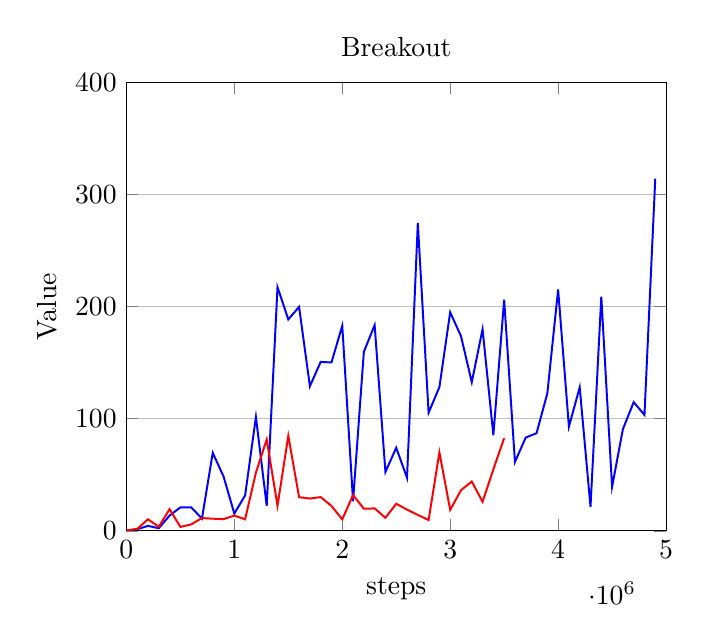
\begin{tikzpicture}

\begin{axis}[%
legend entries={rl-only-small-net,L2-reg,parallel-fs-50-no-aug}, 
legend columns=2,
title=Breakout,
legend to name=named,
legend style={legend cell align=left},
%%width=10in,
%%height=5in,
%%at={(2.596in,2.358in)},
% scale only axis,
xmin=0,
xmax=5000000,
xlabel style={font=\color{white!15!black}},
xlabel={steps},
xlabel near ticks,
ymin=0,
ymax=400,
ylabel style={font=\color{white!15!black}},
ylabel={Value},
ylabel near ticks,
ymajorgrids,
% %scale=0.5,
%%scale=0.4,
axis background/.style={fill=white},
%legend columns=2,
%legend=south outside
]
\addplot [color=blue, line width = 0.25mm]
                table[row sep=crcr]{
                  0 0.20000000298023224\\ 
100000 1.399999976158142\\ 
200000 4.400000095367432\\ 
300000 2.299999952316284\\ 
400000 13.600000381469727\\ 
500000 20.899999618530273\\ 
600000 21.0\\ 
700000 10.899999618530273\\ 
800000 69.5999984741211\\ 
900000 48.5\\ 
1000000 15.399999618530273\\ 
1100000 31.600000381469727\\ 
1200000 101.5999984741211\\ 
1300000 22.399999618530273\\ 
1400000 217.39999389648438\\ 
1500000 188.60000610351562\\ 
1600000 199.8000030517578\\ 
1700000 129.0\\ 
1800000 150.6999969482422\\ 
1900000 150.1999969482422\\ 
2000000 183.0\\ 
2100000 26.399999618530273\\ 
2200000 159.6999969482422\\ 
2300000 183.5\\ 
2400000 52.5\\ 
2500000 74.0999984741211\\ 
2600000 47.29999923706055\\ 
2700000 274.6000061035156\\ 
2800000 105.4000015258789\\ 
2900000 128.1999969482422\\ 
3000000 195.0\\ 
3100000 173.6999969482422\\ 
3200000 132.60000610351562\\ 
3300000 179.89999389648438\\ 
3400000 85.19999694824219\\ 
3500000 206.1999969482422\\ 
3600000 61.5\\ 
3700000 83.19999694824219\\ 
3800000 87.0999984741211\\ 
3900000 122.5999984741211\\ 
4000000 215.3000030517578\\ 
4100000 92.9000015258789\\ 
4200000 128.0\\ 
4300000 21.399999618530273\\ 
4400000 208.89999389648438\\ 
4500000 39.20000076293945\\ 
4600000 90.5999984741211\\ 
4700000 114.80000305175781\\ 
4800000 103.4000015258789\\ 
4900000 314.20001220703125\\ 
};
\addplot [color=red, line width = 0.25mm]
                table[row sep=crcr]{
                  0 0.4000000059604645\\ 
100000 1.7000000476837158\\ 
200000 10.300000190734863\\ 
300000 3.5999999046325684\\ 
400000 19.299999237060547\\ 
500000 3.5\\ 
600000 5.699999809265137\\ 
700000 11.399999618530273\\ 
800000 10.800000190734863\\ 
900000 10.399999618530273\\ 
1000000 13.600000381469727\\ 
1100000 10.300000190734863\\ 
1200000 51.900001525878906\\ 
1300000 81.5\\ 
1400000 22.299999237060547\\ 
1500000 84.69999694824219\\ 
1600000 30.0\\ 
1700000 28.799999237060547\\ 
1800000 30.100000381469727\\ 
1900000 22.200000762939453\\ 
2000000 10.199999809265137\\ 
2100000 31.899999618530273\\ 
2200000 19.700000762939453\\ 
2300000 20.0\\ 
2400000 11.600000381469727\\ 
2500000 24.200000762939453\\ 
2600000 18.899999618530273\\ 
2700000 14.199999809265137\\ 
2800000 9.600000381469727\\ 
2900000 70.0\\ 
3000000 18.700000762939453\\ 
3100000 36.20000076293945\\ 
3200000 44.0\\ 
3300000 25.899999618530273\\ 
3400000 54.900001525878906\\ 
3500000 82.69999694824219\\ 
};
\addplot [color=yellow, line width = 0.25mm]
                table[row sep=crcr]{
                  0 0.800000011920929\\ 
};
\end{axis}
\end{tikzpicture}}}
    \subfloat[]{  \resizebox{0.4\textwidth}{!}{
%\definecolor{blue}{RGB}{76,100,135}
%\definecolor{red}{RGB}{153,0,0}
%\definecolor{yellow}{RGB}{227,178,60}
%\definecolor{mycolor1}{rgb}{0.00000,0.44700,0.74100}%
%\definecolor{mycolor2}{rgb}{0.85000,0.32500,0.09800}%
%\definecolor{mycolor3}{rgb}{0.92900,0.69400,0.12500}%
%
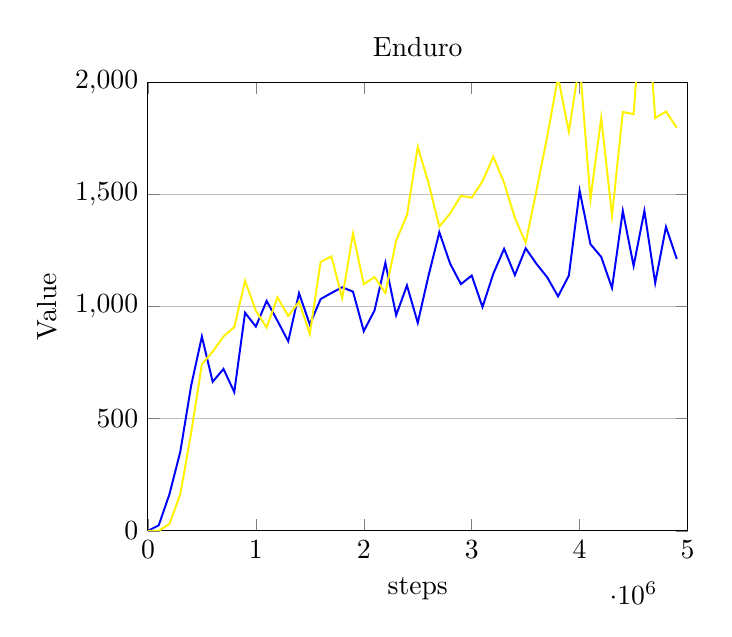
\begin{tikzpicture}

\begin{axis}[%
title=Enduro,
% %width=4.634in,
%%width=10in,
%%height=5in,
%at={(2.596in,2.358in)},
% scale only axis,
xmin=0,
xmax=5000000,
xlabel style={font=\color{white!15!black}},
xlabel={steps},
xlabel near ticks,
ymin=0,
ymax=2000,
ylabel style={font=\color{white!15!black}},
ylabel={Value},
ylabel near ticks,
ymajorgrids,
% %scale=0.5,
%scale=0.4,
axis background/.style={fill=white},
%legend style={legend cell align=left, align=left, draw=white!15!black}
]
\addplot [color=blue, line width = 0.25mm]
                table[row sep=crcr]{
                  0 0.0\\ 
100000 24.299999237060547\\ 
200000 164.3000030517578\\ 
300000 353.0\\ 
400000 646.4000244140625\\ 
500000 866.7000122070312\\ 
600000 664.7000122070312\\ 
700000 722.2000122070312\\ 
800000 618.9000244140625\\ 
900000 972.7999877929688\\ 
1000000 910.9000244140625\\ 
1100000 1025.699951171875\\ 
1200000 937.0\\ 
1300000 845.5999755859375\\ 
1400000 1059.9000244140625\\ 
1500000 920.2999877929688\\ 
1600000 1033.800048828125\\ 
1700000 1061.0\\ 
1800000 1086.5999755859375\\ 
1900000 1066.9000244140625\\ 
2000000 890.9000244140625\\ 
2100000 983.5\\ 
2200000 1195.300048828125\\ 
2300000 962.0\\ 
2400000 1094.800048828125\\ 
2500000 928.0\\ 
2600000 1138.5999755859375\\ 
2700000 1332.300048828125\\ 
2800000 1191.800048828125\\ 
2900000 1100.5999755859375\\ 
3000000 1138.800048828125\\ 
3100000 998.2999877929688\\ 
3200000 1146.800048828125\\ 
3300000 1258.0999755859375\\ 
3400000 1141.0\\ 
3500000 1260.300048828125\\ 
3600000 1190.800048828125\\ 
3700000 1130.5999755859375\\ 
3800000 1046.0999755859375\\ 
3900000 1138.4000244140625\\ 
4000000 1517.5\\ 
4100000 1278.9000244140625\\ 
4200000 1221.699951171875\\ 
4300000 1083.199951171875\\ 
4400000 1426.9000244140625\\ 
4500000 1181.5999755859375\\ 
4600000 1427.199951171875\\ 
4700000 1105.800048828125\\ 
4800000 1355.800048828125\\ 
4900000 1212.9000244140625\\ 
};
\addplot [color=red, line width = 0.25mm]
                table[row sep=crcr]{
                  0 0.0\\ 
};
\addplot [color=yellow, line width = 0.25mm]
                table[row sep=crcr]{
                  0 0.0\\ 
100000 0.0\\ 
200000 30.700000762939453\\ 
300000 163.6999969482422\\ 
400000 435.79998779296875\\ 
500000 743.2000122070312\\ 
600000 799.2000122070312\\ 
700000 867.0\\ 
800000 908.4000244140625\\ 
900000 1115.300048828125\\ 
1000000 981.4000244140625\\ 
1100000 906.9000244140625\\ 
1200000 1041.5999755859375\\ 
1300000 958.5999755859375\\ 
1400000 1021.9000244140625\\ 
1500000 877.7000122070312\\ 
1600000 1199.4000244140625\\ 
1700000 1224.0\\ 
1800000 1038.199951171875\\ 
1900000 1326.0999755859375\\ 
2000000 1100.0\\ 
2100000 1132.0999755859375\\ 
2200000 1060.9000244140625\\ 
2300000 1294.300048828125\\ 
2400000 1407.699951171875\\ 
2500000 1712.5\\ 
2600000 1551.5\\ 
2700000 1357.0\\ 
2800000 1415.800048828125\\ 
2900000 1494.5\\ 
3000000 1486.0\\ 
3100000 1559.699951171875\\ 
3200000 1668.5\\ 
3300000 1552.800048828125\\ 
3400000 1395.800048828125\\ 
3500000 1284.9000244140625\\ 
3600000 1518.0\\ 
3700000 1759.5999755859375\\ 
3800000 2024.9000244140625\\ 
3900000 1780.0999755859375\\ 
4000000 2090.5\\ 
4100000 1479.0999755859375\\ 
4200000 1841.699951171875\\ 
4300000 1405.5999755859375\\ 
4400000 1868.300048828125\\ 
4500000 1858.699951171875\\ 
4600000 2527.0\\ 
4700000 1841.0\\ 
4800000 1870.800048828125\\ 
4900000 1797.9000244140625\\ 
};
\end{axis}
\end{tikzpicture}}}\\
  \vspace{-1cm}
    \subfloat[]{  \resizebox{0.4\textwidth}{!}{
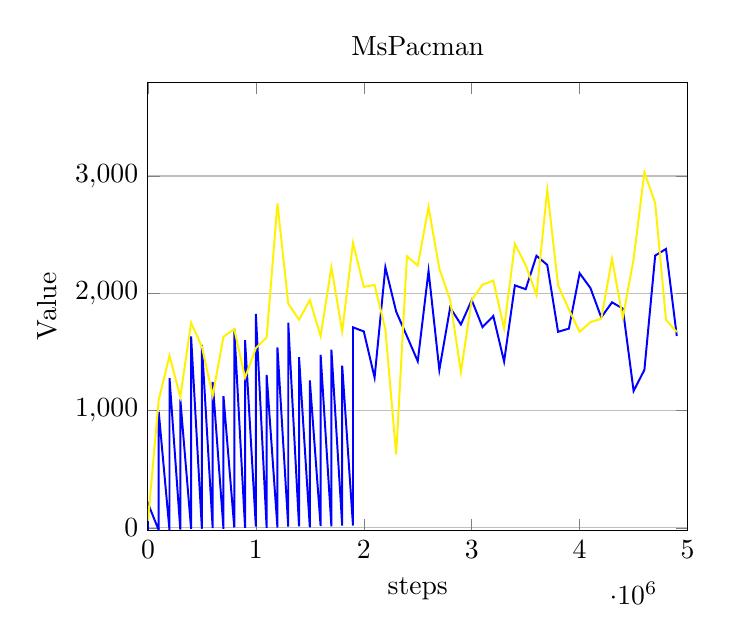
\begin{tikzpicture}

\begin{axis}[%
title=MsPacman,
% %width=4.634in,
%width=10in,
%height=5in,
%at={(2.596in,2.358in)},
% scale only axis,
xmin=0,
xmax=5000000,
xlabel style={font=\color{white!15!black}},
xlabel={steps},
xlabel near ticks,
ymin=-22,
ymax=3800,
ylabel style={font=\color{white!15!black}},
ylabel={Value},
ylabel near ticks,
ymajorgrids,
% %scale=0.5,
%scale=0.4,
axis background/.style={fill=white},
%legend style={legend cell align=left, align=left, draw=white!15!black}
]
\addplot [color=blue, line width = 0.25mm]
                table[row sep=crcr]{
                  0 -21.0\\ 
0 210.0\\ 
100000 -19.799999237060547\\ 
100000 990.0\\ 
200000 -20.700000762939453\\ 
200000 1277.0\\ 
300000 -15.0\\ 
300000 1096.0\\ 
400000 -7.0\\ 
400000 1632.0\\ 
500000 -6.900000095367432\\ 
500000 1561.0\\ 
600000 -1.899999976158142\\ 
600000 1245.0\\ 
700000 -7.599999904632568\\ 
700000 1123.0\\ 
800000 4.0\\ 
800000 1696.0\\ 
900000 1.5\\ 
900000 1600.0\\ 
1000000 11.300000190734863\\ 
1000000 1824.0\\ 
1100000 1.2000000476837158\\ 
1100000 1304.0\\ 
1200000 3.700000047683716\\ 
1200000 1538.0\\ 
1300000 11.5\\ 
1300000 1750.0\\ 
1400000 13.600000381469727\\ 
1400000 1456.0\\ 
1500000 5.699999809265137\\ 
1500000 1258.0\\ 
1600000 15.600000381469727\\ 
1600000 1476.0\\ 
1700000 13.5\\ 
1700000 1519.0\\ 
1800000 19.299999237060547\\ 
1800000 1383.0\\ 
1900000 20.799999237060547\\ 
1900000 1710.0\\ 
2000000 1675.0\\ 
2100000 1282.0\\ 
2200000 2222.0\\ 
2300000 1844.0\\ 
2400000 1634.0\\ 
2500000 1421.0\\ 
2600000 2191.0\\ 
2700000 1347.0\\ 
2800000 1878.0\\ 
2900000 1735.0\\ 
3000000 1942.0\\ 
3100000 1712.0\\ 
3200000 1806.0\\ 
3300000 1419.0\\ 
3400000 2068.0\\ 
3500000 2035.0\\ 
3600000 2320.0\\ 
3700000 2242.0\\ 
3800000 1672.0\\ 
3900000 1699.0\\ 
4000000 2171.0\\ 
4100000 2045.0\\ 
4200000 1795.0\\ 
4300000 1923.0\\ 
4400000 1870.0\\ 
4500000 1167.0\\ 
4600000 1348.0\\ 
4700000 2322.0\\ 
4800000 2378.0\\ 
4900000 1636.0\\ 
};
\addplot [color=red, line width = 0.25mm]
                table[row sep=crcr]{
                  0 0.0\\ 
};
\addplot [color=yellow, line width = 0.25mm]
                table[row sep=crcr]{
                  0 60.0\\ 
100000 1090.0\\ 
200000 1469.0\\ 
300000 1117.0\\ 
400000 1749.0\\ 
500000 1545.0\\ 
600000 1128.0\\ 
700000 1630.0\\ 
800000 1695.0\\ 
900000 1281.0\\ 
1000000 1532.0\\ 
1100000 1625.0\\ 
1200000 2767.0\\ 
1300000 1912.0\\ 
1400000 1775.0\\ 
1500000 1942.0\\ 
1600000 1636.0\\ 
1700000 2222.0\\ 
1800000 1676.0\\ 
1900000 2430.0\\ 
2000000 2055.0\\ 
2100000 2072.0\\ 
2200000 1693.0\\ 
2300000 625.0\\ 
2400000 2317.0\\ 
2500000 2236.0\\ 
2600000 2736.0\\ 
2700000 2209.0\\ 
2800000 1944.0\\ 
2900000 1329.0\\ 
3000000 1944.0\\ 
3100000 2074.0\\ 
3200000 2109.0\\ 
3300000 1701.0\\ 
3400000 2421.0\\ 
3500000 2240.0\\ 
3600000 1986.0\\ 
3700000 2883.0\\ 
3800000 2069.0\\ 
3900000 1863.0\\ 
4000000 1672.0\\ 
4100000 1754.0\\ 
4200000 1783.0\\ 
4300000 2293.0\\ 
4400000 1791.0\\ 
4500000 2293.0\\ 
4600000 3033.0\\ 
4700000 2768.0\\ 
4800000 1774.0\\ 
4900000 1670.0\\ 
};
\end{axis}
\end{tikzpicture}}}
    \subfloat[]{  \resizebox{0.4\textwidth}{!}{
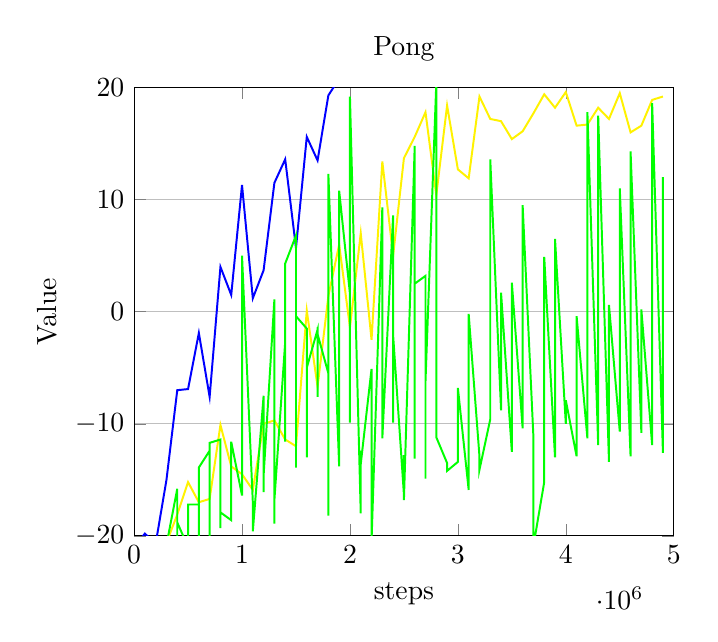
\begin{tikzpicture}

\begin{axis}[%
title=Pong,
% %width=4.634in,
%width=10in,
%height=5in,
%at={(2.596in,2.358in)},
% scale only axis,
xmin=0,
xmax=5000000,
xlabel style={font=\color{white!15!black}},
xlabel={steps},
xlabel near ticks,
ymin=-20,
ymax=20,
ylabel style={font=\color{white!15!black}},
ylabel={Value},
ylabel near ticks,
ymajorgrids,
% %scale=0.5,
%scale=0.4,
axis background/.style={fill=white},
%legend style={legend cell align=left, align=left, draw=white!15!black}
]
\addplot [color=blue, line width = 0.25mm]
                table[row sep=crcr]{
                  0 -21.0\\ 
100000 -19.799999237060547\\ 
200000 -20.700000762939453\\ 
300000 -15.0\\ 
400000 -7.0\\ 
500000 -6.900000095367432\\ 
600000 -1.899999976158142\\ 
700000 -7.599999904632568\\ 
800000 4.0\\ 
900000 1.5\\ 
1000000 11.300000190734863\\ 
1100000 1.2000000476837158\\ 
1200000 3.700000047683716\\ 
1300000 11.5\\ 
1400000 13.600000381469727\\ 
1500000 5.699999809265137\\ 
1600000 15.600000381469727\\ 
1700000 13.5\\ 
1800000 19.299999237060547\\ 
1900000 20.799999237060547\\ 
};
\addplot [color=red, line width = 0.25mm]
                table[row sep=crcr]{
                  0 0.0\\ 
};
\addplot [color=yellow, line width = 0.25mm]
                table[row sep=crcr]{
                  0 -21.0\\ 
0 -21.0\\ 
0 -21.0\\ 
100000 -21.0\\ 
200000 -20.299999237060547\\ 
300000 -20.600000381469727\\ 
400000 -18.100000381469727\\ 
500000 -15.199999809265137\\ 
600000 -17.0\\ 
700000 -16.700000762939453\\ 
800000 -10.100000381469727\\ 
900000 -13.800000190734863\\ 
1000000 -14.5\\ 
1100000 -15.899999618530273\\ 
1200000 -10.0\\ 
1300000 -9.699999809265137\\ 
1400000 -11.399999618530273\\ 
1500000 -12.0\\ 
1600000 0.10000000149011612\\ 
1700000 -6.699999809265137\\ 
1800000 1.399999976158142\\ 
1900000 6.0\\ 
2000000 -1.399999976158142\\ 
2100000 7.0\\ 
2200000 -2.5\\ 
2300000 13.399999618530273\\ 
2400000 5.0\\ 
2500000 13.699999809265137\\ 
2600000 15.600000381469727\\ 
2700000 17.799999237060547\\ 
2800000 10.399999618530273\\ 
2900000 18.399999618530273\\ 
3000000 12.699999809265137\\ 
3100000 11.899999618530273\\ 
3200000 19.200000762939453\\ 
3300000 17.200000762939453\\ 
3400000 17.0\\ 
3500000 15.399999618530273\\ 
3600000 16.100000381469727\\ 
3700000 17.700000762939453\\ 
3800000 19.399999618530273\\ 
3900000 18.200000762939453\\ 
4000000 19.600000381469727\\ 
4100000 16.600000381469727\\ 
4200000 16.700000762939453\\ 
4300000 18.200000762939453\\ 
4400000 17.200000762939453\\ 
4500000 19.5\\ 
4600000 16.0\\ 
4700000 16.600000381469727\\ 
4800000 18.899999618530273\\ 
4900000 19.200000762939453\\ 
};
\addplot [color=green, line width = 0.25mm]
                table[row sep=crcr]{
                  0 -21.0\\ 
0 -21.0\\ 
0 -21.0\\ 
0 -21.0\\ 
100000 -21.0\\ 
100000 -20.600000381469727\\ 
100000 -21.0\\ 
200000 -20.399999618530273\\ 
200000 -21.0\\ 
200000 -20.799999237060547\\ 
300000 -20.600000381469727\\ 
300000 -20.799999237060547\\ 
300000 -20.799999237060547\\ 
400000 -15.800000190734863\\ 
400000 -20.399999618530273\\ 
400000 -18.799999237060547\\ 
500000 -21.0\\ 
500000 -21.0\\ 
500000 -17.200000762939453\\ 
600000 -17.200000762939453\\ 
600000 -20.600000381469727\\ 
600000 -13.899999618530273\\ 
700000 -12.399999618530273\\ 
700000 -20.100000381469727\\ 
700000 -11.699999809265137\\ 
800000 -11.399999618530273\\ 
800000 -19.299999237060547\\ 
800000 -17.899999618530273\\ 
900000 -18.600000381469727\\ 
900000 -15.699999809265137\\ 
900000 -11.600000381469727\\ 
1000000 -16.399999618530273\\ 
1000000 -16.0\\ 
1000000 5.0\\ 
1100000 -17.0\\ 
1100000 -17.5\\ 
1100000 -19.600000381469727\\ 
1200000 -7.5\\ 
1200000 -16.100000381469727\\ 
1200000 -14.600000381469727\\ 
1300000 1.100000023841858\\ 
1300000 -18.899999618530273\\ 
1300000 -16.799999237060547\\ 
1400000 -2.700000047683716\\ 
1400000 -11.600000381469727\\ 
1400000 4.300000190734863\\ 
1500000 6.800000190734863\\ 
1500000 -13.899999618530273\\ 
1500000 -0.4000000059604645\\ 
1600000 -1.5\\ 
1600000 -13.0\\ 
1600000 -5.0\\ 
1700000 -1.600000023841858\\ 
1700000 -7.599999904632568\\ 
1700000 -2.0\\ 
1800000 -5.5\\ 
1800000 -18.200000762939453\\ 
1800000 12.300000190734863\\ 
1900000 -13.800000190734863\\ 
1900000 -10.0\\ 
1900000 10.800000190734863\\ 
2000000 1.600000023841858\\ 
2000000 -9.899999618530273\\ 
2000000 19.200000762939453\\ 
2100000 -18.0\\ 
2100000 -12.399999618530273\\ 
2100000 -13.600000381469727\\ 
2200000 -5.099999904632568\\ 
2200000 -13.899999618530273\\ 
2200000 -20.5\\ 
2300000 9.300000190734863\\ 
2300000 -8.199999809265137\\ 
2300000 -11.300000190734863\\ 
2400000 8.600000381469727\\ 
2400000 -9.899999618530273\\ 
2400000 -2.0999999046325684\\ 
2500000 -16.299999237060547\\ 
2500000 -12.800000190734863\\ 
2500000 -16.799999237060547\\ 
2600000 14.800000190734863\\ 
2600000 -13.100000381469727\\ 
2600000 2.5\\ 
2700000 3.200000047683716\\ 
2700000 -14.899999618530273\\ 
2700000 -6.199999809265137\\ 
2800000 20.399999618530273\\ 
2800000 -9.800000190734863\\ 
2800000 -11.199999809265137\\ 
2900000 -13.5\\ 
2900000 -14.199999809265137\\ 
3000000 -13.399999618530273\\ 
3000000 -6.800000190734863\\ 
3100000 -15.899999618530273\\ 
3100000 -0.20000000298023224\\ 
3200000 -12.899999618530273\\ 
3200000 -14.100000381469727\\ 
3300000 -9.600000381469727\\ 
3300000 13.600000381469727\\ 
3400000 -8.800000190734863\\ 
3400000 1.7000000476837158\\ 
3500000 -12.5\\ 
3500000 2.5999999046325684\\ 
3600000 -10.399999618530273\\ 
3600000 9.5\\ 
3700000 -11.199999809265137\\ 
3700000 -20.899999618530273\\ 
3800000 -15.199999809265137\\ 
3800000 4.900000095367432\\ 
3900000 -13.0\\ 
3900000 6.5\\ 
4000000 -10.0\\ 
4000000 -7.900000095367432\\ 
4100000 -12.899999618530273\\ 
4100000 -0.4000000059604645\\ 
4200000 -11.300000190734863\\ 
4200000 17.799999237060547\\ 
4300000 -11.899999618530273\\ 
4300000 17.5\\ 
4400000 -13.399999618530273\\ 
4400000 0.6000000238418579\\ 
4500000 -10.699999809265137\\ 
4500000 11.0\\ 
4600000 -12.899999618530273\\ 
4600000 14.300000190734863\\ 
4700000 -10.800000190734863\\ 
4700000 0.20000000298023224\\ 
4800000 -11.899999618530273\\ 
4800000 18.600000381469727\\ 
4900000 -12.600000381469727\\ 
4900000 12.0\\ 
};
\end{axis}
\end{tikzpicture}}}\\
  \vspace{-1cm}
    \subfloat[]{  \resizebox{0.4\textwidth}{!}{
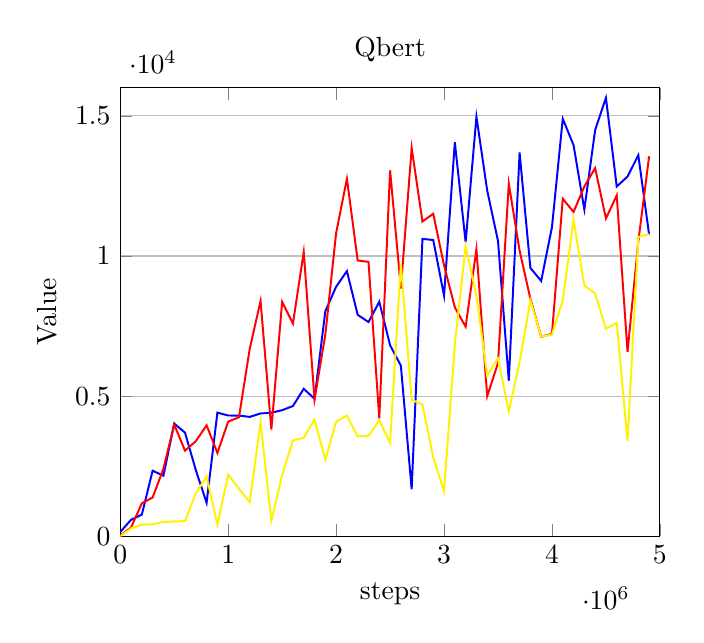
\begin{tikzpicture}

\begin{axis}[%
title=Qbert,
% %width=4.634in,
%width=10in,
%height=5in,
%at={(2.596in,2.358in)},
% scale only axis,
xmin=0,
xmax=5000000,
xlabel style={font=\color{white!15!black}},
xlabel={steps},
xlabel near ticks,
ymin=0,
ymax=16000,
ylabel style={font=\color{white!15!black}},
ylabel={Value},
ylabel near ticks,
ymajorgrids,
% %scale=0.5,
%scale=0.4,
axis background/.style={fill=white},
%legend style={legend cell align=left, align=left, draw=white!15!black}
]
\addplot [color=blue, line width = 0.25mm]
                table[row sep=crcr]{
                  0 150.0\\ 
100000 585.0\\ 
200000 772.5\\ 
300000 2337.5\\ 
400000 2157.5\\ 
500000 4022.5\\ 
600000 3695.0\\ 
700000 2362.5\\ 
800000 1192.5\\ 
900000 4410.0\\ 
1000000 4307.5\\ 
1100000 4305.0\\ 
1200000 4257.5\\ 
1300000 4380.0\\ 
1400000 4407.5\\ 
1500000 4497.5\\ 
1600000 4645.0\\ 
1700000 5260.0\\ 
1800000 4905.0\\ 
1900000 8030.0\\ 
2000000 8902.5\\ 
2100000 9460.0\\ 
2200000 7900.0\\ 
2300000 7642.5\\ 
2400000 8367.5\\ 
2500000 6815.0\\ 
2600000 6085.0\\ 
2700000 1677.5\\ 
2800000 10610.0\\ 
2900000 10570.0\\ 
3000000 8585.0\\ 
3100000 14057.5\\ 
3200000 10490.0\\ 
3300000 14970.0\\ 
3400000 12332.5\\ 
3500000 10537.5\\ 
3600000 5550.0\\ 
3700000 13692.5\\ 
3800000 9572.5\\ 
3900000 9110.0\\ 
4000000 11030.0\\ 
4100000 14897.5\\ 
4200000 13955.0\\ 
4300000 11660.0\\ 
4400000 14495.0\\ 
4500000 15645.0\\ 
4600000 12480.0\\ 
4700000 12835.0\\ 
4800000 13597.5\\ 
4900000 10762.5\\ 
};
\addplot [color=red, line width = 0.25mm]
                table[row sep=crcr]{
                  0 22.5\\ 
100000 310.0\\ 
200000 1172.5\\ 
300000 1382.5\\ 
400000 2410.0\\ 
500000 3982.5\\ 
600000 3052.5\\ 
700000 3390.0\\ 
800000 3957.5\\ 
900000 2970.0\\ 
1000000 4090.0\\ 
1100000 4245.0\\ 
1200000 6697.5\\ 
1300000 8395.0\\ 
1400000 3807.5\\ 
1500000 8360.0\\ 
1600000 7590.0\\ 
1700000 10142.5\\ 
1800000 4877.5\\ 
1900000 7190.0\\ 
2000000 10817.5\\ 
2100000 12755.0\\ 
2200000 9840.0\\ 
2300000 9790.0\\ 
2400000 4202.5\\ 
2500000 13057.5\\ 
2600000 8842.5\\ 
2700000 13852.5\\ 
2800000 11230.0\\ 
2900000 11507.5\\ 
3000000 9665.0\\ 
3100000 8167.5\\ 
3200000 7475.0\\ 
3300000 10242.5\\ 
3400000 4997.5\\ 
3500000 6180.0\\ 
3600000 12582.5\\ 
3700000 10190.0\\ 
3800000 8475.0\\ 
3900000 7115.0\\ 
4000000 7222.5\\ 
4100000 12042.5\\ 
4200000 11572.5\\ 
4300000 12480.0\\ 
4400000 13137.5\\ 
4500000 11337.5\\ 
4600000 12165.0\\ 
4700000 6580.0\\ 
4800000 10517.5\\ 
4900000 13560.0\\ 
};
\addplot [color=yellow, line width = 0.25mm]
                table[row sep=crcr]{
                  0 0.0\\ 
100000 280.0\\ 
200000 415.0\\ 
300000 425.0\\ 
400000 507.5\\ 
500000 525.0\\ 
600000 537.5\\ 
700000 1525.0\\ 
800000 2137.5\\ 
900000 407.5\\ 
1000000 2195.0\\ 
1100000 1690.0\\ 
1200000 1215.0\\ 
1300000 4077.5\\ 
1400000 550.0\\ 
1500000 2185.0\\ 
1600000 3417.5\\ 
1700000 3512.5\\ 
1800000 4165.0\\ 
1900000 2730.0\\ 
2000000 4090.0\\ 
2100000 4305.0\\ 
2200000 3557.5\\ 
2300000 3585.0\\ 
2400000 4137.5\\ 
2500000 3335.0\\ 
2600000 9722.5\\ 
2700000 4865.0\\ 
2800000 4700.0\\ 
2900000 2812.5\\ 
3000000 1605.0\\ 
3100000 6847.5\\ 
3200000 10342.5\\ 
3300000 8590.0\\ 
3400000 5732.5\\ 
3500000 6345.0\\ 
3600000 4447.5\\ 
3700000 6217.5\\ 
3800000 8415.0\\ 
3900000 7120.0\\ 
4000000 7195.0\\ 
4100000 8415.0\\ 
4200000 11307.5\\ 
4300000 8942.5\\ 
4400000 8662.5\\ 
4500000 7402.5\\ 
4600000 7612.5\\ 
4700000 3395.0\\ 
4800000 10680.0\\ 
4900000 10780.0\\ 
};
\end{axis}
\end{tikzpicture}}}
    \subfloat[]{  \resizebox{0.4\textwidth}{!}{
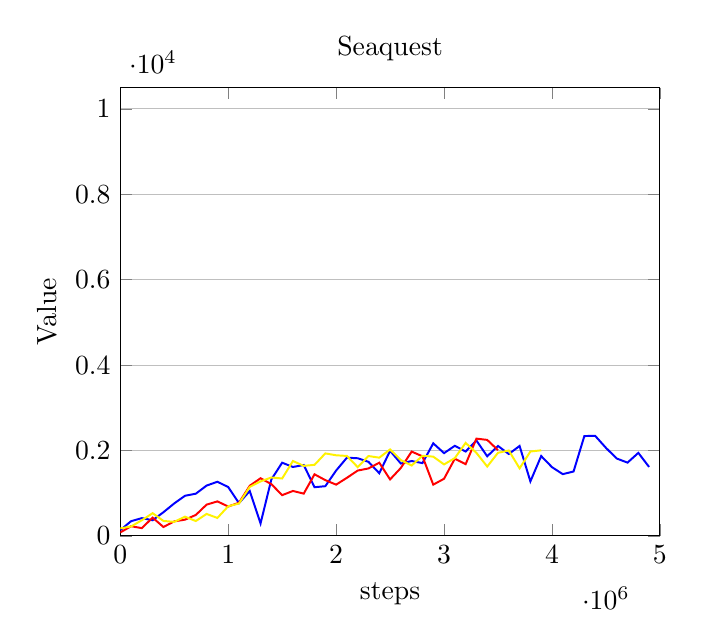
\begin{tikzpicture}

\begin{axis}[%
title=Seaquest,
% %width=4.634in,
%width=10in,
%height=5in,
%at={(2.596in,2.358in)},
% scale only axis,
xmin=0,
xmax=5000000,
xlabel style={font=\color{white!15!black}},
xlabel={steps},
xlabel near ticks,
ymin=0,
ymax=10500,
ylabel style={font=\color{white!15!black}},
ylabel={Value},
ylabel near ticks,
ymajorgrids,
% %scale=0.5,
%scale=0.4,
axis background/.style={fill=white},
%legend style={legend cell align=left, align=left, draw=white!15!black}
]
\addplot [color=blue, line width = 0.25mm]
                table[row sep=crcr]{
                  0 134.0\\ 
100000 344.0\\ 
200000 416.0\\ 
300000 366.0\\ 
400000 554.0\\ 
500000 760.0\\ 
600000 940.0\\ 
700000 988.0\\ 
800000 1178.0\\ 
900000 1268.0\\ 
1000000 1144.0\\ 
1100000 768.0\\ 
1200000 1052.0\\ 
1300000 292.0\\ 
1400000 1322.0\\ 
1500000 1714.0\\ 
1600000 1614.0\\ 
1700000 1660.0\\ 
1800000 1140.0\\ 
1900000 1164.0\\ 
2000000 1530.0\\ 
2100000 1832.0\\ 
2200000 1818.0\\ 
2300000 1734.0\\ 
2400000 1468.0\\ 
2500000 1992.0\\ 
2600000 1694.0\\ 
2700000 1754.0\\ 
2800000 1704.0\\ 
2900000 2168.0\\ 
3000000 1938.0\\ 
3100000 2110.0\\ 
3200000 1976.0\\ 
3300000 2234.0\\ 
3400000 1864.0\\ 
3500000 2106.0\\ 
3600000 1918.0\\ 
3700000 2106.0\\ 
3800000 1276.0\\ 
3900000 1870.0\\ 
4000000 1610.0\\ 
4100000 1446.0\\ 
4200000 1508.0\\ 
4300000 2338.0\\ 
4400000 2344.0\\ 
4500000 2062.0\\ 
4600000 1812.0\\ 
4700000 1716.0\\ 
4800000 1944.0\\ 
4900000 1614.0\\ 
};
\addplot [color=red, line width = 0.25mm]
                table[row sep=crcr]{
                  0 80.0\\ 
100000 226.0\\ 
200000 182.0\\ 
300000 428.0\\ 
400000 208.0\\ 
500000 340.0\\ 
600000 380.0\\ 
700000 490.0\\ 
800000 732.0\\ 
900000 808.0\\ 
1000000 688.0\\ 
1100000 776.0\\ 
1200000 1174.0\\ 
1300000 1350.0\\ 
1400000 1212.0\\ 
1500000 954.0\\ 
1600000 1052.0\\ 
1700000 990.0\\ 
1800000 1442.0\\ 
1900000 1306.0\\ 
2000000 1200.0\\ 
2100000 1360.0\\ 
2200000 1530.0\\ 
2300000 1580.0\\ 
2400000 1714.0\\ 
2500000 1322.0\\ 
2600000 1592.0\\ 
2700000 1974.0\\ 
2800000 1864.0\\ 
2900000 1200.0\\ 
3000000 1338.0\\ 
3100000 1808.0\\ 
3200000 1680.0\\ 
3300000 2278.0\\ 
3400000 2248.0\\ 
3500000 2008.0\\ 
};
\addplot [color=yellow, line width = 0.25mm]
                table[row sep=crcr]{
                  0 176.0\\ 
100000 220.0\\ 
200000 366.0\\ 
300000 532.0\\ 
400000 350.0\\ 
500000 328.0\\ 
600000 450.0\\ 
700000 348.0\\ 
800000 514.0\\ 
900000 420.0\\ 
1000000 694.0\\ 
1100000 758.0\\ 
1200000 1148.0\\ 
1300000 1276.0\\ 
1400000 1368.0\\ 
1500000 1344.0\\ 
1600000 1754.0\\ 
1700000 1640.0\\ 
1800000 1664.0\\ 
1900000 1932.0\\ 
2000000 1888.0\\ 
2100000 1872.0\\ 
2200000 1610.0\\ 
2300000 1870.0\\ 
2400000 1832.0\\ 
2500000 2024.0\\ 
2600000 1774.0\\ 
2700000 1648.0\\ 
2800000 1876.0\\ 
2900000 1856.0\\ 
3000000 1674.0\\ 
3100000 1822.0\\ 
3200000 2178.0\\ 
3300000 1944.0\\ 
3400000 1624.0\\ 
3500000 1946.0\\ 
3600000 2000.0\\ 
3700000 1582.0\\ 
3800000 1976.0\\ 
3900000 2004.0\\ 
};
\end{axis}
\end{tikzpicture}}}\\
  \vspace{-1cm}
    \subfloat[]{  \resizebox{0.4\textwidth}{!}{
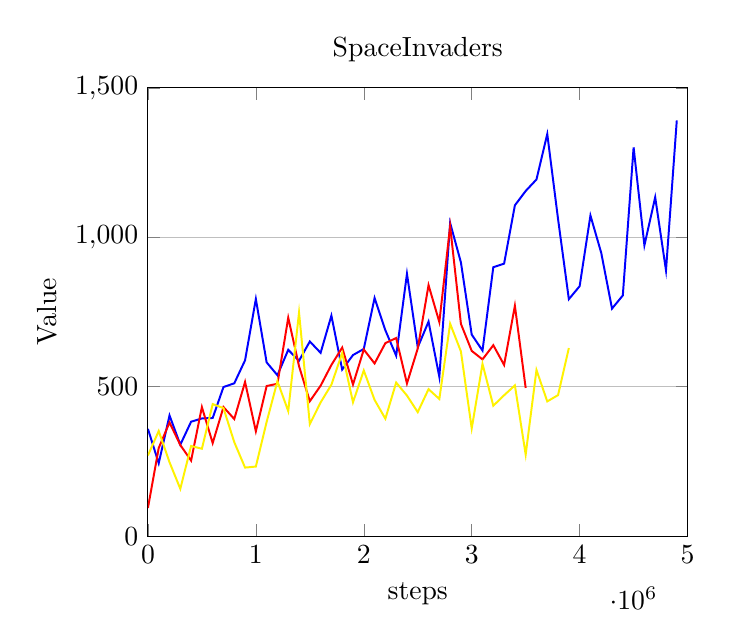
\begin{tikzpicture}

\begin{axis}[%
title=SpaceInvaders,
%width=10in,
%height=5in,
%at={(2.596in,2.358in)},
% scale only axis,
xmin=0,
xmax=5000000,
xlabel style={font=\color{white!15!black}},
xlabel={steps},
xlabel near ticks,
ymin=0,
ymax=1500,
ylabel style={font=\color{white!15!black}},
ylabel={Value},
ylabel near ticks,
ymajorgrids,
% %scale=0.5,
%scale=0.4,
axis background/.style={fill=white},
%legend style={legend cell align=left, align=left, draw=white!15!black}
]
\addplot [color=blue, line width = 0.25mm]
                table[row sep=crcr]{
                  0 359.0\\ 
100000 244.0\\ 
200000 404.0\\ 
300000 306.0\\ 
400000 383.0\\ 
500000 394.0\\ 
600000 395.5\\ 
700000 499.0\\ 
800000 511.5\\ 
900000 588.5\\ 
1000000 793.5\\ 
1100000 581.5\\ 
1200000 538.5\\ 
1300000 623.5\\ 
1400000 587.0\\ 
1500000 651.5\\ 
1600000 613.5\\ 
1700000 738.0\\ 
1800000 557.5\\ 
1900000 606.0\\ 
2000000 626.5\\ 
2100000 797.0\\ 
2200000 689.0\\ 
2300000 604.0\\ 
2400000 878.0\\ 
2500000 632.0\\ 
2600000 718.0\\ 
2700000 533.0\\ 
2800000 1048.0\\ 
2900000 916.0\\ 
3000000 674.5\\ 
3100000 621.0\\ 
3200000 900.0\\ 
3300000 912.0\\ 
3400000 1107.0\\ 
3500000 1155.0\\ 
3600000 1193.5\\ 
3700000 1345.5\\ 
3800000 1061.0\\ 
3900000 793.0\\ 
4000000 836.5\\ 
4100000 1073.0\\ 
4200000 948.0\\ 
4300000 761.5\\ 
4400000 805.5\\ 
4500000 1301.0\\ 
4600000 973.0\\ 
4700000 1134.0\\ 
4800000 889.5\\ 
4900000 1391.0\\ 
};
\addplot [color=red, line width = 0.25mm]
                table[row sep=crcr]{
                  0 94.5\\ 
100000 295.0\\ 
200000 380.5\\ 
300000 305.0\\ 
400000 253.0\\ 
500000 432.0\\ 
600000 311.5\\ 
700000 432.0\\ 
800000 392.0\\ 
900000 516.0\\ 
1000000 351.0\\ 
1100000 502.5\\ 
1200000 510.0\\ 
1300000 731.0\\ 
1400000 569.0\\ 
1500000 451.5\\ 
1600000 503.5\\ 
1700000 573.0\\ 
1800000 631.0\\ 
1900000 507.5\\ 
2000000 624.5\\ 
2100000 578.0\\ 
2200000 646.0\\ 
2300000 663.0\\ 
2400000 511.0\\ 
2500000 628.0\\ 
2600000 840.0\\ 
2700000 716.5\\ 
2800000 1037.0\\ 
2900000 710.5\\ 
3000000 620.0\\ 
3100000 591.5\\ 
3200000 639.0\\ 
3300000 573.0\\ 
3400000 771.0\\ 
3500000 496.0\\ 
};
\addplot [color=yellow, line width = 0.25mm]
                table[row sep=crcr]{
                  0 270.0\\ 
100000 352.0\\ 
200000 247.5\\ 
300000 158.5\\ 
400000 302.0\\ 
500000 292.5\\ 
600000 442.0\\ 
700000 428.5\\ 
800000 314.5\\ 
900000 229.5\\ 
1000000 233.0\\ 
1100000 382.5\\ 
1200000 518.5\\ 
1300000 418.5\\ 
1400000 748.5\\ 
1500000 375.0\\ 
1600000 447.5\\ 
1700000 507.0\\ 
1800000 613.0\\ 
1900000 448.0\\ 
2000000 554.5\\ 
2100000 456.0\\ 
2200000 393.0\\ 
2300000 514.0\\ 
2400000 470.5\\ 
2500000 415.0\\ 
2600000 492.0\\ 
2700000 459.0\\ 
2800000 711.0\\ 
2900000 618.0\\ 
3000000 360.5\\ 
3100000 576.5\\ 
3200000 436.5\\ 
3300000 471.5\\ 
3400000 504.5\\ 
3500000 273.0\\ 
3600000 556.0\\ 
3700000 451.0\\ 
3800000 472.0\\ 
3900000 629.5\\ 
};
\end{axis}
\end{tikzpicture}}}
    \\

    \ref{named}
  \caption{Runs with Rainbow only, but with different encoder sizes. As can be seen,
  some games strongly benefit from having a larger encoder, while learning
fails on others.}
  \label{fig:big-vs-small-enc-rl-only}
\end{figure}

As can be seen in \ref{fig:big-vs-small-enc-rl-only}, some games benefit greatly from
having a large encoder (ex. Seaquest), while learning completely fails on others 
(ex. Breakout).
Despite rising the variance of the final result, the effect seems to be neutral
overall.



\section{Effectiveness of continuous updates}
Having seen the effect of having pretrained encoders, we turn the attention
to the effect of continuous updating of the encoder with reconstruction loss.
The results are shown in \ref{fig-parallel}.

\begin{figure}[!t]
  \captionsetup[subfloat]{position=top,labelformat=empty}
  \centering

    \subfloat[]{  \resizebox{0.4\textwidth}{!}{
%\definecolor{blue}{RGB}{76,100,135}
%\definecolor{red}{RGB}{153,0,0}
%\definecolor{yellow}{RGB}{227,178,60}
%\definecolor{mycolor1}{rgb}{0.00000,0.44700,0.74100}%
%\definecolor{mycolor2}{rgb}{0.85000,0.32500,0.09800}%
%\definecolor{mycolor3}{rgb}{0.92900,0.69400,0.12500}%
%
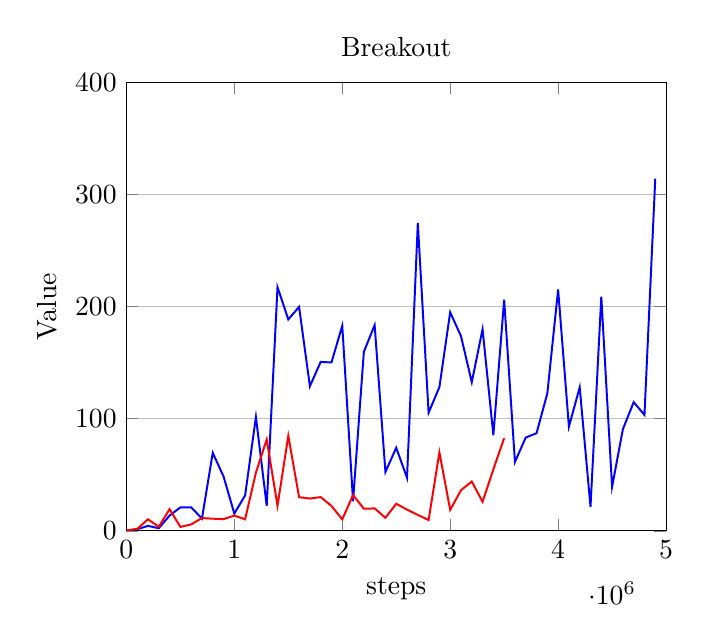
\begin{tikzpicture}

\begin{axis}[%
legend entries={rl-only-small-net,L2-reg,parallel-fs-50-no-aug}, 
legend columns=2,
title=Breakout,
legend to name=named,
legend style={legend cell align=left},
%%width=10in,
%%height=5in,
%%at={(2.596in,2.358in)},
% scale only axis,
xmin=0,
xmax=5000000,
xlabel style={font=\color{white!15!black}},
xlabel={steps},
xlabel near ticks,
ymin=0,
ymax=400,
ylabel style={font=\color{white!15!black}},
ylabel={Value},
ylabel near ticks,
ymajorgrids,
% %scale=0.5,
%%scale=0.4,
axis background/.style={fill=white},
%legend columns=2,
%legend=south outside
]
\addplot [color=blue, line width = 0.25mm]
                table[row sep=crcr]{
                  0 0.20000000298023224\\ 
100000 1.399999976158142\\ 
200000 4.400000095367432\\ 
300000 2.299999952316284\\ 
400000 13.600000381469727\\ 
500000 20.899999618530273\\ 
600000 21.0\\ 
700000 10.899999618530273\\ 
800000 69.5999984741211\\ 
900000 48.5\\ 
1000000 15.399999618530273\\ 
1100000 31.600000381469727\\ 
1200000 101.5999984741211\\ 
1300000 22.399999618530273\\ 
1400000 217.39999389648438\\ 
1500000 188.60000610351562\\ 
1600000 199.8000030517578\\ 
1700000 129.0\\ 
1800000 150.6999969482422\\ 
1900000 150.1999969482422\\ 
2000000 183.0\\ 
2100000 26.399999618530273\\ 
2200000 159.6999969482422\\ 
2300000 183.5\\ 
2400000 52.5\\ 
2500000 74.0999984741211\\ 
2600000 47.29999923706055\\ 
2700000 274.6000061035156\\ 
2800000 105.4000015258789\\ 
2900000 128.1999969482422\\ 
3000000 195.0\\ 
3100000 173.6999969482422\\ 
3200000 132.60000610351562\\ 
3300000 179.89999389648438\\ 
3400000 85.19999694824219\\ 
3500000 206.1999969482422\\ 
3600000 61.5\\ 
3700000 83.19999694824219\\ 
3800000 87.0999984741211\\ 
3900000 122.5999984741211\\ 
4000000 215.3000030517578\\ 
4100000 92.9000015258789\\ 
4200000 128.0\\ 
4300000 21.399999618530273\\ 
4400000 208.89999389648438\\ 
4500000 39.20000076293945\\ 
4600000 90.5999984741211\\ 
4700000 114.80000305175781\\ 
4800000 103.4000015258789\\ 
4900000 314.20001220703125\\ 
};
\addplot [color=red, line width = 0.25mm]
                table[row sep=crcr]{
                  0 0.4000000059604645\\ 
100000 1.7000000476837158\\ 
200000 10.300000190734863\\ 
300000 3.5999999046325684\\ 
400000 19.299999237060547\\ 
500000 3.5\\ 
600000 5.699999809265137\\ 
700000 11.399999618530273\\ 
800000 10.800000190734863\\ 
900000 10.399999618530273\\ 
1000000 13.600000381469727\\ 
1100000 10.300000190734863\\ 
1200000 51.900001525878906\\ 
1300000 81.5\\ 
1400000 22.299999237060547\\ 
1500000 84.69999694824219\\ 
1600000 30.0\\ 
1700000 28.799999237060547\\ 
1800000 30.100000381469727\\ 
1900000 22.200000762939453\\ 
2000000 10.199999809265137\\ 
2100000 31.899999618530273\\ 
2200000 19.700000762939453\\ 
2300000 20.0\\ 
2400000 11.600000381469727\\ 
2500000 24.200000762939453\\ 
2600000 18.899999618530273\\ 
2700000 14.199999809265137\\ 
2800000 9.600000381469727\\ 
2900000 70.0\\ 
3000000 18.700000762939453\\ 
3100000 36.20000076293945\\ 
3200000 44.0\\ 
3300000 25.899999618530273\\ 
3400000 54.900001525878906\\ 
3500000 82.69999694824219\\ 
};
\addplot [color=yellow, line width = 0.25mm]
                table[row sep=crcr]{
                  0 0.800000011920929\\ 
};
\end{axis}
\end{tikzpicture}}}
    \subfloat[]{  \resizebox{0.4\textwidth}{!}{
%\definecolor{blue}{RGB}{76,100,135}
%\definecolor{red}{RGB}{153,0,0}
%\definecolor{yellow}{RGB}{227,178,60}
%\definecolor{mycolor1}{rgb}{0.00000,0.44700,0.74100}%
%\definecolor{mycolor2}{rgb}{0.85000,0.32500,0.09800}%
%\definecolor{mycolor3}{rgb}{0.92900,0.69400,0.12500}%
%
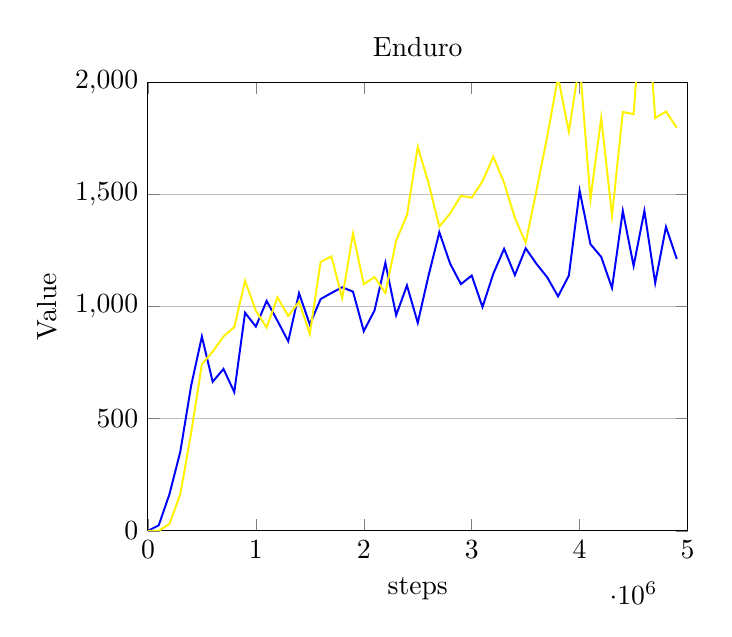
\begin{tikzpicture}

\begin{axis}[%
title=Enduro,
% %width=4.634in,
%%width=10in,
%%height=5in,
%at={(2.596in,2.358in)},
% scale only axis,
xmin=0,
xmax=5000000,
xlabel style={font=\color{white!15!black}},
xlabel={steps},
xlabel near ticks,
ymin=0,
ymax=2000,
ylabel style={font=\color{white!15!black}},
ylabel={Value},
ylabel near ticks,
ymajorgrids,
% %scale=0.5,
%scale=0.4,
axis background/.style={fill=white},
%legend style={legend cell align=left, align=left, draw=white!15!black}
]
\addplot [color=blue, line width = 0.25mm]
                table[row sep=crcr]{
                  0 0.0\\ 
100000 24.299999237060547\\ 
200000 164.3000030517578\\ 
300000 353.0\\ 
400000 646.4000244140625\\ 
500000 866.7000122070312\\ 
600000 664.7000122070312\\ 
700000 722.2000122070312\\ 
800000 618.9000244140625\\ 
900000 972.7999877929688\\ 
1000000 910.9000244140625\\ 
1100000 1025.699951171875\\ 
1200000 937.0\\ 
1300000 845.5999755859375\\ 
1400000 1059.9000244140625\\ 
1500000 920.2999877929688\\ 
1600000 1033.800048828125\\ 
1700000 1061.0\\ 
1800000 1086.5999755859375\\ 
1900000 1066.9000244140625\\ 
2000000 890.9000244140625\\ 
2100000 983.5\\ 
2200000 1195.300048828125\\ 
2300000 962.0\\ 
2400000 1094.800048828125\\ 
2500000 928.0\\ 
2600000 1138.5999755859375\\ 
2700000 1332.300048828125\\ 
2800000 1191.800048828125\\ 
2900000 1100.5999755859375\\ 
3000000 1138.800048828125\\ 
3100000 998.2999877929688\\ 
3200000 1146.800048828125\\ 
3300000 1258.0999755859375\\ 
3400000 1141.0\\ 
3500000 1260.300048828125\\ 
3600000 1190.800048828125\\ 
3700000 1130.5999755859375\\ 
3800000 1046.0999755859375\\ 
3900000 1138.4000244140625\\ 
4000000 1517.5\\ 
4100000 1278.9000244140625\\ 
4200000 1221.699951171875\\ 
4300000 1083.199951171875\\ 
4400000 1426.9000244140625\\ 
4500000 1181.5999755859375\\ 
4600000 1427.199951171875\\ 
4700000 1105.800048828125\\ 
4800000 1355.800048828125\\ 
4900000 1212.9000244140625\\ 
};
\addplot [color=red, line width = 0.25mm]
                table[row sep=crcr]{
                  0 0.0\\ 
};
\addplot [color=yellow, line width = 0.25mm]
                table[row sep=crcr]{
                  0 0.0\\ 
100000 0.0\\ 
200000 30.700000762939453\\ 
300000 163.6999969482422\\ 
400000 435.79998779296875\\ 
500000 743.2000122070312\\ 
600000 799.2000122070312\\ 
700000 867.0\\ 
800000 908.4000244140625\\ 
900000 1115.300048828125\\ 
1000000 981.4000244140625\\ 
1100000 906.9000244140625\\ 
1200000 1041.5999755859375\\ 
1300000 958.5999755859375\\ 
1400000 1021.9000244140625\\ 
1500000 877.7000122070312\\ 
1600000 1199.4000244140625\\ 
1700000 1224.0\\ 
1800000 1038.199951171875\\ 
1900000 1326.0999755859375\\ 
2000000 1100.0\\ 
2100000 1132.0999755859375\\ 
2200000 1060.9000244140625\\ 
2300000 1294.300048828125\\ 
2400000 1407.699951171875\\ 
2500000 1712.5\\ 
2600000 1551.5\\ 
2700000 1357.0\\ 
2800000 1415.800048828125\\ 
2900000 1494.5\\ 
3000000 1486.0\\ 
3100000 1559.699951171875\\ 
3200000 1668.5\\ 
3300000 1552.800048828125\\ 
3400000 1395.800048828125\\ 
3500000 1284.9000244140625\\ 
3600000 1518.0\\ 
3700000 1759.5999755859375\\ 
3800000 2024.9000244140625\\ 
3900000 1780.0999755859375\\ 
4000000 2090.5\\ 
4100000 1479.0999755859375\\ 
4200000 1841.699951171875\\ 
4300000 1405.5999755859375\\ 
4400000 1868.300048828125\\ 
4500000 1858.699951171875\\ 
4600000 2527.0\\ 
4700000 1841.0\\ 
4800000 1870.800048828125\\ 
4900000 1797.9000244140625\\ 
};
\end{axis}
\end{tikzpicture}}}\\
  \vspace{-1cm}
    \subfloat[]{  \resizebox{0.4\textwidth}{!}{
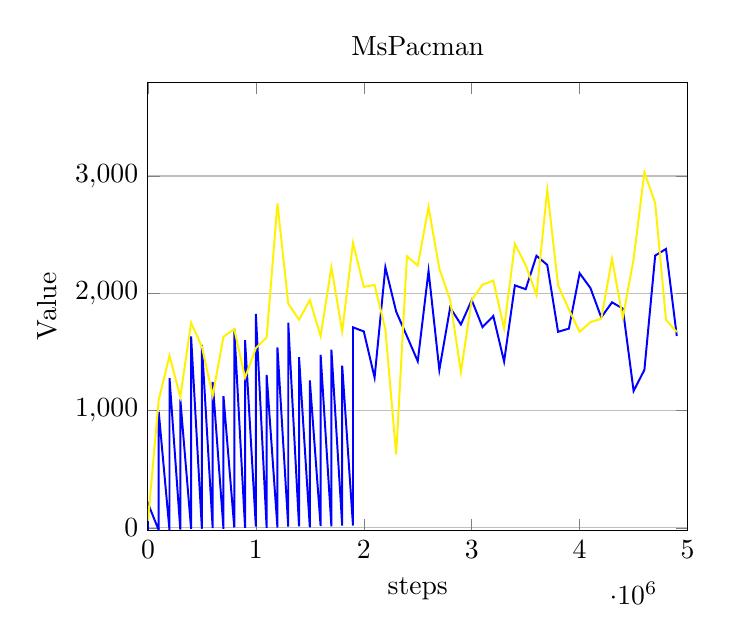
\begin{tikzpicture}

\begin{axis}[%
title=MsPacman,
% %width=4.634in,
%width=10in,
%height=5in,
%at={(2.596in,2.358in)},
% scale only axis,
xmin=0,
xmax=5000000,
xlabel style={font=\color{white!15!black}},
xlabel={steps},
xlabel near ticks,
ymin=-22,
ymax=3800,
ylabel style={font=\color{white!15!black}},
ylabel={Value},
ylabel near ticks,
ymajorgrids,
% %scale=0.5,
%scale=0.4,
axis background/.style={fill=white},
%legend style={legend cell align=left, align=left, draw=white!15!black}
]
\addplot [color=blue, line width = 0.25mm]
                table[row sep=crcr]{
                  0 -21.0\\ 
0 210.0\\ 
100000 -19.799999237060547\\ 
100000 990.0\\ 
200000 -20.700000762939453\\ 
200000 1277.0\\ 
300000 -15.0\\ 
300000 1096.0\\ 
400000 -7.0\\ 
400000 1632.0\\ 
500000 -6.900000095367432\\ 
500000 1561.0\\ 
600000 -1.899999976158142\\ 
600000 1245.0\\ 
700000 -7.599999904632568\\ 
700000 1123.0\\ 
800000 4.0\\ 
800000 1696.0\\ 
900000 1.5\\ 
900000 1600.0\\ 
1000000 11.300000190734863\\ 
1000000 1824.0\\ 
1100000 1.2000000476837158\\ 
1100000 1304.0\\ 
1200000 3.700000047683716\\ 
1200000 1538.0\\ 
1300000 11.5\\ 
1300000 1750.0\\ 
1400000 13.600000381469727\\ 
1400000 1456.0\\ 
1500000 5.699999809265137\\ 
1500000 1258.0\\ 
1600000 15.600000381469727\\ 
1600000 1476.0\\ 
1700000 13.5\\ 
1700000 1519.0\\ 
1800000 19.299999237060547\\ 
1800000 1383.0\\ 
1900000 20.799999237060547\\ 
1900000 1710.0\\ 
2000000 1675.0\\ 
2100000 1282.0\\ 
2200000 2222.0\\ 
2300000 1844.0\\ 
2400000 1634.0\\ 
2500000 1421.0\\ 
2600000 2191.0\\ 
2700000 1347.0\\ 
2800000 1878.0\\ 
2900000 1735.0\\ 
3000000 1942.0\\ 
3100000 1712.0\\ 
3200000 1806.0\\ 
3300000 1419.0\\ 
3400000 2068.0\\ 
3500000 2035.0\\ 
3600000 2320.0\\ 
3700000 2242.0\\ 
3800000 1672.0\\ 
3900000 1699.0\\ 
4000000 2171.0\\ 
4100000 2045.0\\ 
4200000 1795.0\\ 
4300000 1923.0\\ 
4400000 1870.0\\ 
4500000 1167.0\\ 
4600000 1348.0\\ 
4700000 2322.0\\ 
4800000 2378.0\\ 
4900000 1636.0\\ 
};
\addplot [color=red, line width = 0.25mm]
                table[row sep=crcr]{
                  0 0.0\\ 
};
\addplot [color=yellow, line width = 0.25mm]
                table[row sep=crcr]{
                  0 60.0\\ 
100000 1090.0\\ 
200000 1469.0\\ 
300000 1117.0\\ 
400000 1749.0\\ 
500000 1545.0\\ 
600000 1128.0\\ 
700000 1630.0\\ 
800000 1695.0\\ 
900000 1281.0\\ 
1000000 1532.0\\ 
1100000 1625.0\\ 
1200000 2767.0\\ 
1300000 1912.0\\ 
1400000 1775.0\\ 
1500000 1942.0\\ 
1600000 1636.0\\ 
1700000 2222.0\\ 
1800000 1676.0\\ 
1900000 2430.0\\ 
2000000 2055.0\\ 
2100000 2072.0\\ 
2200000 1693.0\\ 
2300000 625.0\\ 
2400000 2317.0\\ 
2500000 2236.0\\ 
2600000 2736.0\\ 
2700000 2209.0\\ 
2800000 1944.0\\ 
2900000 1329.0\\ 
3000000 1944.0\\ 
3100000 2074.0\\ 
3200000 2109.0\\ 
3300000 1701.0\\ 
3400000 2421.0\\ 
3500000 2240.0\\ 
3600000 1986.0\\ 
3700000 2883.0\\ 
3800000 2069.0\\ 
3900000 1863.0\\ 
4000000 1672.0\\ 
4100000 1754.0\\ 
4200000 1783.0\\ 
4300000 2293.0\\ 
4400000 1791.0\\ 
4500000 2293.0\\ 
4600000 3033.0\\ 
4700000 2768.0\\ 
4800000 1774.0\\ 
4900000 1670.0\\ 
};
\end{axis}
\end{tikzpicture}}}
    \subfloat[]{  \resizebox{0.4\textwidth}{!}{
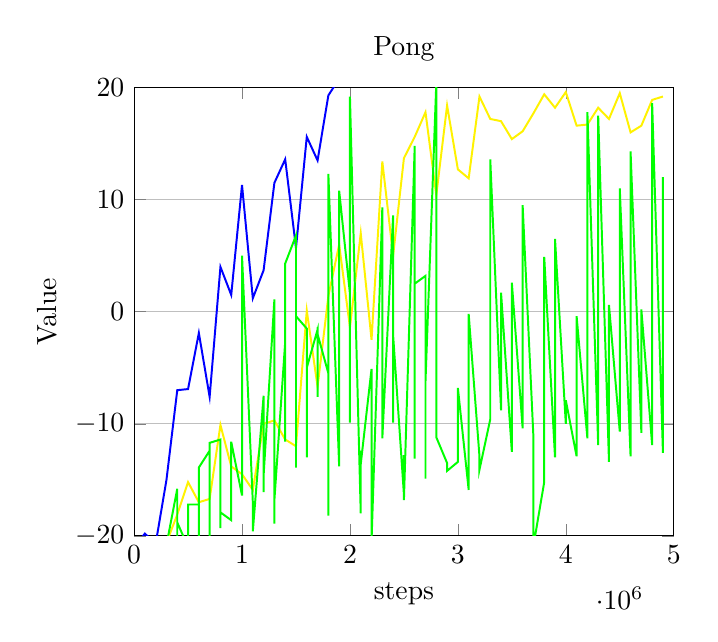
\begin{tikzpicture}

\begin{axis}[%
title=Pong,
% %width=4.634in,
%width=10in,
%height=5in,
%at={(2.596in,2.358in)},
% scale only axis,
xmin=0,
xmax=5000000,
xlabel style={font=\color{white!15!black}},
xlabel={steps},
xlabel near ticks,
ymin=-20,
ymax=20,
ylabel style={font=\color{white!15!black}},
ylabel={Value},
ylabel near ticks,
ymajorgrids,
% %scale=0.5,
%scale=0.4,
axis background/.style={fill=white},
%legend style={legend cell align=left, align=left, draw=white!15!black}
]
\addplot [color=blue, line width = 0.25mm]
                table[row sep=crcr]{
                  0 -21.0\\ 
100000 -19.799999237060547\\ 
200000 -20.700000762939453\\ 
300000 -15.0\\ 
400000 -7.0\\ 
500000 -6.900000095367432\\ 
600000 -1.899999976158142\\ 
700000 -7.599999904632568\\ 
800000 4.0\\ 
900000 1.5\\ 
1000000 11.300000190734863\\ 
1100000 1.2000000476837158\\ 
1200000 3.700000047683716\\ 
1300000 11.5\\ 
1400000 13.600000381469727\\ 
1500000 5.699999809265137\\ 
1600000 15.600000381469727\\ 
1700000 13.5\\ 
1800000 19.299999237060547\\ 
1900000 20.799999237060547\\ 
};
\addplot [color=red, line width = 0.25mm]
                table[row sep=crcr]{
                  0 0.0\\ 
};
\addplot [color=yellow, line width = 0.25mm]
                table[row sep=crcr]{
                  0 -21.0\\ 
0 -21.0\\ 
0 -21.0\\ 
100000 -21.0\\ 
200000 -20.299999237060547\\ 
300000 -20.600000381469727\\ 
400000 -18.100000381469727\\ 
500000 -15.199999809265137\\ 
600000 -17.0\\ 
700000 -16.700000762939453\\ 
800000 -10.100000381469727\\ 
900000 -13.800000190734863\\ 
1000000 -14.5\\ 
1100000 -15.899999618530273\\ 
1200000 -10.0\\ 
1300000 -9.699999809265137\\ 
1400000 -11.399999618530273\\ 
1500000 -12.0\\ 
1600000 0.10000000149011612\\ 
1700000 -6.699999809265137\\ 
1800000 1.399999976158142\\ 
1900000 6.0\\ 
2000000 -1.399999976158142\\ 
2100000 7.0\\ 
2200000 -2.5\\ 
2300000 13.399999618530273\\ 
2400000 5.0\\ 
2500000 13.699999809265137\\ 
2600000 15.600000381469727\\ 
2700000 17.799999237060547\\ 
2800000 10.399999618530273\\ 
2900000 18.399999618530273\\ 
3000000 12.699999809265137\\ 
3100000 11.899999618530273\\ 
3200000 19.200000762939453\\ 
3300000 17.200000762939453\\ 
3400000 17.0\\ 
3500000 15.399999618530273\\ 
3600000 16.100000381469727\\ 
3700000 17.700000762939453\\ 
3800000 19.399999618530273\\ 
3900000 18.200000762939453\\ 
4000000 19.600000381469727\\ 
4100000 16.600000381469727\\ 
4200000 16.700000762939453\\ 
4300000 18.200000762939453\\ 
4400000 17.200000762939453\\ 
4500000 19.5\\ 
4600000 16.0\\ 
4700000 16.600000381469727\\ 
4800000 18.899999618530273\\ 
4900000 19.200000762939453\\ 
};
\addplot [color=green, line width = 0.25mm]
                table[row sep=crcr]{
                  0 -21.0\\ 
0 -21.0\\ 
0 -21.0\\ 
0 -21.0\\ 
100000 -21.0\\ 
100000 -20.600000381469727\\ 
100000 -21.0\\ 
200000 -20.399999618530273\\ 
200000 -21.0\\ 
200000 -20.799999237060547\\ 
300000 -20.600000381469727\\ 
300000 -20.799999237060547\\ 
300000 -20.799999237060547\\ 
400000 -15.800000190734863\\ 
400000 -20.399999618530273\\ 
400000 -18.799999237060547\\ 
500000 -21.0\\ 
500000 -21.0\\ 
500000 -17.200000762939453\\ 
600000 -17.200000762939453\\ 
600000 -20.600000381469727\\ 
600000 -13.899999618530273\\ 
700000 -12.399999618530273\\ 
700000 -20.100000381469727\\ 
700000 -11.699999809265137\\ 
800000 -11.399999618530273\\ 
800000 -19.299999237060547\\ 
800000 -17.899999618530273\\ 
900000 -18.600000381469727\\ 
900000 -15.699999809265137\\ 
900000 -11.600000381469727\\ 
1000000 -16.399999618530273\\ 
1000000 -16.0\\ 
1000000 5.0\\ 
1100000 -17.0\\ 
1100000 -17.5\\ 
1100000 -19.600000381469727\\ 
1200000 -7.5\\ 
1200000 -16.100000381469727\\ 
1200000 -14.600000381469727\\ 
1300000 1.100000023841858\\ 
1300000 -18.899999618530273\\ 
1300000 -16.799999237060547\\ 
1400000 -2.700000047683716\\ 
1400000 -11.600000381469727\\ 
1400000 4.300000190734863\\ 
1500000 6.800000190734863\\ 
1500000 -13.899999618530273\\ 
1500000 -0.4000000059604645\\ 
1600000 -1.5\\ 
1600000 -13.0\\ 
1600000 -5.0\\ 
1700000 -1.600000023841858\\ 
1700000 -7.599999904632568\\ 
1700000 -2.0\\ 
1800000 -5.5\\ 
1800000 -18.200000762939453\\ 
1800000 12.300000190734863\\ 
1900000 -13.800000190734863\\ 
1900000 -10.0\\ 
1900000 10.800000190734863\\ 
2000000 1.600000023841858\\ 
2000000 -9.899999618530273\\ 
2000000 19.200000762939453\\ 
2100000 -18.0\\ 
2100000 -12.399999618530273\\ 
2100000 -13.600000381469727\\ 
2200000 -5.099999904632568\\ 
2200000 -13.899999618530273\\ 
2200000 -20.5\\ 
2300000 9.300000190734863\\ 
2300000 -8.199999809265137\\ 
2300000 -11.300000190734863\\ 
2400000 8.600000381469727\\ 
2400000 -9.899999618530273\\ 
2400000 -2.0999999046325684\\ 
2500000 -16.299999237060547\\ 
2500000 -12.800000190734863\\ 
2500000 -16.799999237060547\\ 
2600000 14.800000190734863\\ 
2600000 -13.100000381469727\\ 
2600000 2.5\\ 
2700000 3.200000047683716\\ 
2700000 -14.899999618530273\\ 
2700000 -6.199999809265137\\ 
2800000 20.399999618530273\\ 
2800000 -9.800000190734863\\ 
2800000 -11.199999809265137\\ 
2900000 -13.5\\ 
2900000 -14.199999809265137\\ 
3000000 -13.399999618530273\\ 
3000000 -6.800000190734863\\ 
3100000 -15.899999618530273\\ 
3100000 -0.20000000298023224\\ 
3200000 -12.899999618530273\\ 
3200000 -14.100000381469727\\ 
3300000 -9.600000381469727\\ 
3300000 13.600000381469727\\ 
3400000 -8.800000190734863\\ 
3400000 1.7000000476837158\\ 
3500000 -12.5\\ 
3500000 2.5999999046325684\\ 
3600000 -10.399999618530273\\ 
3600000 9.5\\ 
3700000 -11.199999809265137\\ 
3700000 -20.899999618530273\\ 
3800000 -15.199999809265137\\ 
3800000 4.900000095367432\\ 
3900000 -13.0\\ 
3900000 6.5\\ 
4000000 -10.0\\ 
4000000 -7.900000095367432\\ 
4100000 -12.899999618530273\\ 
4100000 -0.4000000059604645\\ 
4200000 -11.300000190734863\\ 
4200000 17.799999237060547\\ 
4300000 -11.899999618530273\\ 
4300000 17.5\\ 
4400000 -13.399999618530273\\ 
4400000 0.6000000238418579\\ 
4500000 -10.699999809265137\\ 
4500000 11.0\\ 
4600000 -12.899999618530273\\ 
4600000 14.300000190734863\\ 
4700000 -10.800000190734863\\ 
4700000 0.20000000298023224\\ 
4800000 -11.899999618530273\\ 
4800000 18.600000381469727\\ 
4900000 -12.600000381469727\\ 
4900000 12.0\\ 
};
\end{axis}
\end{tikzpicture}}}\\
  \vspace{-1cm}
    \subfloat[]{  \resizebox{0.4\textwidth}{!}{
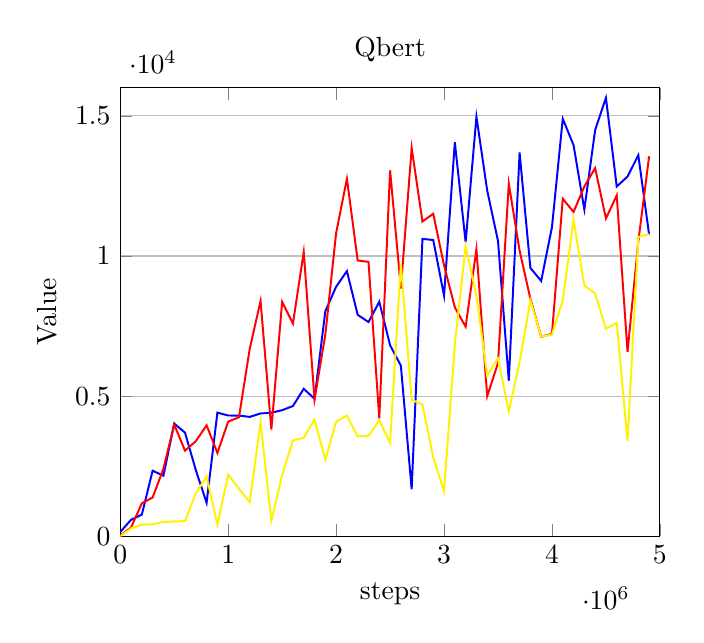
\begin{tikzpicture}

\begin{axis}[%
title=Qbert,
% %width=4.634in,
%width=10in,
%height=5in,
%at={(2.596in,2.358in)},
% scale only axis,
xmin=0,
xmax=5000000,
xlabel style={font=\color{white!15!black}},
xlabel={steps},
xlabel near ticks,
ymin=0,
ymax=16000,
ylabel style={font=\color{white!15!black}},
ylabel={Value},
ylabel near ticks,
ymajorgrids,
% %scale=0.5,
%scale=0.4,
axis background/.style={fill=white},
%legend style={legend cell align=left, align=left, draw=white!15!black}
]
\addplot [color=blue, line width = 0.25mm]
                table[row sep=crcr]{
                  0 150.0\\ 
100000 585.0\\ 
200000 772.5\\ 
300000 2337.5\\ 
400000 2157.5\\ 
500000 4022.5\\ 
600000 3695.0\\ 
700000 2362.5\\ 
800000 1192.5\\ 
900000 4410.0\\ 
1000000 4307.5\\ 
1100000 4305.0\\ 
1200000 4257.5\\ 
1300000 4380.0\\ 
1400000 4407.5\\ 
1500000 4497.5\\ 
1600000 4645.0\\ 
1700000 5260.0\\ 
1800000 4905.0\\ 
1900000 8030.0\\ 
2000000 8902.5\\ 
2100000 9460.0\\ 
2200000 7900.0\\ 
2300000 7642.5\\ 
2400000 8367.5\\ 
2500000 6815.0\\ 
2600000 6085.0\\ 
2700000 1677.5\\ 
2800000 10610.0\\ 
2900000 10570.0\\ 
3000000 8585.0\\ 
3100000 14057.5\\ 
3200000 10490.0\\ 
3300000 14970.0\\ 
3400000 12332.5\\ 
3500000 10537.5\\ 
3600000 5550.0\\ 
3700000 13692.5\\ 
3800000 9572.5\\ 
3900000 9110.0\\ 
4000000 11030.0\\ 
4100000 14897.5\\ 
4200000 13955.0\\ 
4300000 11660.0\\ 
4400000 14495.0\\ 
4500000 15645.0\\ 
4600000 12480.0\\ 
4700000 12835.0\\ 
4800000 13597.5\\ 
4900000 10762.5\\ 
};
\addplot [color=red, line width = 0.25mm]
                table[row sep=crcr]{
                  0 22.5\\ 
100000 310.0\\ 
200000 1172.5\\ 
300000 1382.5\\ 
400000 2410.0\\ 
500000 3982.5\\ 
600000 3052.5\\ 
700000 3390.0\\ 
800000 3957.5\\ 
900000 2970.0\\ 
1000000 4090.0\\ 
1100000 4245.0\\ 
1200000 6697.5\\ 
1300000 8395.0\\ 
1400000 3807.5\\ 
1500000 8360.0\\ 
1600000 7590.0\\ 
1700000 10142.5\\ 
1800000 4877.5\\ 
1900000 7190.0\\ 
2000000 10817.5\\ 
2100000 12755.0\\ 
2200000 9840.0\\ 
2300000 9790.0\\ 
2400000 4202.5\\ 
2500000 13057.5\\ 
2600000 8842.5\\ 
2700000 13852.5\\ 
2800000 11230.0\\ 
2900000 11507.5\\ 
3000000 9665.0\\ 
3100000 8167.5\\ 
3200000 7475.0\\ 
3300000 10242.5\\ 
3400000 4997.5\\ 
3500000 6180.0\\ 
3600000 12582.5\\ 
3700000 10190.0\\ 
3800000 8475.0\\ 
3900000 7115.0\\ 
4000000 7222.5\\ 
4100000 12042.5\\ 
4200000 11572.5\\ 
4300000 12480.0\\ 
4400000 13137.5\\ 
4500000 11337.5\\ 
4600000 12165.0\\ 
4700000 6580.0\\ 
4800000 10517.5\\ 
4900000 13560.0\\ 
};
\addplot [color=yellow, line width = 0.25mm]
                table[row sep=crcr]{
                  0 0.0\\ 
100000 280.0\\ 
200000 415.0\\ 
300000 425.0\\ 
400000 507.5\\ 
500000 525.0\\ 
600000 537.5\\ 
700000 1525.0\\ 
800000 2137.5\\ 
900000 407.5\\ 
1000000 2195.0\\ 
1100000 1690.0\\ 
1200000 1215.0\\ 
1300000 4077.5\\ 
1400000 550.0\\ 
1500000 2185.0\\ 
1600000 3417.5\\ 
1700000 3512.5\\ 
1800000 4165.0\\ 
1900000 2730.0\\ 
2000000 4090.0\\ 
2100000 4305.0\\ 
2200000 3557.5\\ 
2300000 3585.0\\ 
2400000 4137.5\\ 
2500000 3335.0\\ 
2600000 9722.5\\ 
2700000 4865.0\\ 
2800000 4700.0\\ 
2900000 2812.5\\ 
3000000 1605.0\\ 
3100000 6847.5\\ 
3200000 10342.5\\ 
3300000 8590.0\\ 
3400000 5732.5\\ 
3500000 6345.0\\ 
3600000 4447.5\\ 
3700000 6217.5\\ 
3800000 8415.0\\ 
3900000 7120.0\\ 
4000000 7195.0\\ 
4100000 8415.0\\ 
4200000 11307.5\\ 
4300000 8942.5\\ 
4400000 8662.5\\ 
4500000 7402.5\\ 
4600000 7612.5\\ 
4700000 3395.0\\ 
4800000 10680.0\\ 
4900000 10780.0\\ 
};
\end{axis}
\end{tikzpicture}}}
    \subfloat[]{  \resizebox{0.4\textwidth}{!}{
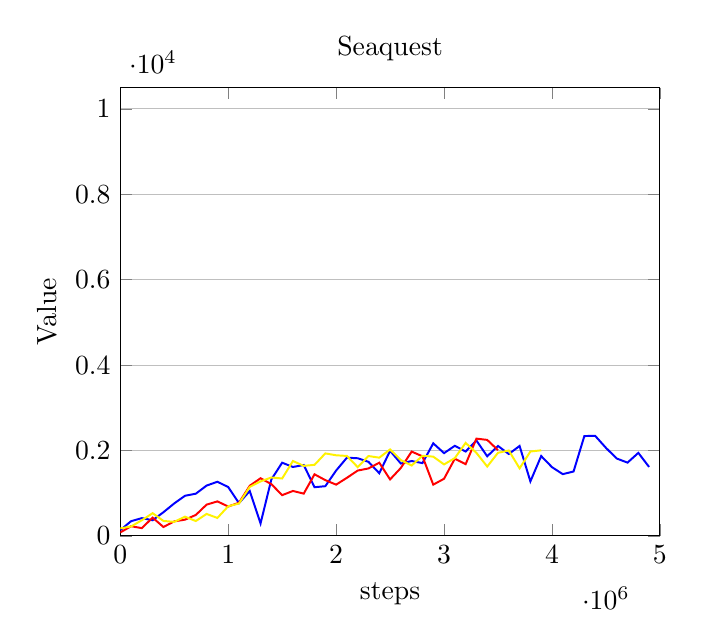
\begin{tikzpicture}

\begin{axis}[%
title=Seaquest,
% %width=4.634in,
%width=10in,
%height=5in,
%at={(2.596in,2.358in)},
% scale only axis,
xmin=0,
xmax=5000000,
xlabel style={font=\color{white!15!black}},
xlabel={steps},
xlabel near ticks,
ymin=0,
ymax=10500,
ylabel style={font=\color{white!15!black}},
ylabel={Value},
ylabel near ticks,
ymajorgrids,
% %scale=0.5,
%scale=0.4,
axis background/.style={fill=white},
%legend style={legend cell align=left, align=left, draw=white!15!black}
]
\addplot [color=blue, line width = 0.25mm]
                table[row sep=crcr]{
                  0 134.0\\ 
100000 344.0\\ 
200000 416.0\\ 
300000 366.0\\ 
400000 554.0\\ 
500000 760.0\\ 
600000 940.0\\ 
700000 988.0\\ 
800000 1178.0\\ 
900000 1268.0\\ 
1000000 1144.0\\ 
1100000 768.0\\ 
1200000 1052.0\\ 
1300000 292.0\\ 
1400000 1322.0\\ 
1500000 1714.0\\ 
1600000 1614.0\\ 
1700000 1660.0\\ 
1800000 1140.0\\ 
1900000 1164.0\\ 
2000000 1530.0\\ 
2100000 1832.0\\ 
2200000 1818.0\\ 
2300000 1734.0\\ 
2400000 1468.0\\ 
2500000 1992.0\\ 
2600000 1694.0\\ 
2700000 1754.0\\ 
2800000 1704.0\\ 
2900000 2168.0\\ 
3000000 1938.0\\ 
3100000 2110.0\\ 
3200000 1976.0\\ 
3300000 2234.0\\ 
3400000 1864.0\\ 
3500000 2106.0\\ 
3600000 1918.0\\ 
3700000 2106.0\\ 
3800000 1276.0\\ 
3900000 1870.0\\ 
4000000 1610.0\\ 
4100000 1446.0\\ 
4200000 1508.0\\ 
4300000 2338.0\\ 
4400000 2344.0\\ 
4500000 2062.0\\ 
4600000 1812.0\\ 
4700000 1716.0\\ 
4800000 1944.0\\ 
4900000 1614.0\\ 
};
\addplot [color=red, line width = 0.25mm]
                table[row sep=crcr]{
                  0 80.0\\ 
100000 226.0\\ 
200000 182.0\\ 
300000 428.0\\ 
400000 208.0\\ 
500000 340.0\\ 
600000 380.0\\ 
700000 490.0\\ 
800000 732.0\\ 
900000 808.0\\ 
1000000 688.0\\ 
1100000 776.0\\ 
1200000 1174.0\\ 
1300000 1350.0\\ 
1400000 1212.0\\ 
1500000 954.0\\ 
1600000 1052.0\\ 
1700000 990.0\\ 
1800000 1442.0\\ 
1900000 1306.0\\ 
2000000 1200.0\\ 
2100000 1360.0\\ 
2200000 1530.0\\ 
2300000 1580.0\\ 
2400000 1714.0\\ 
2500000 1322.0\\ 
2600000 1592.0\\ 
2700000 1974.0\\ 
2800000 1864.0\\ 
2900000 1200.0\\ 
3000000 1338.0\\ 
3100000 1808.0\\ 
3200000 1680.0\\ 
3300000 2278.0\\ 
3400000 2248.0\\ 
3500000 2008.0\\ 
};
\addplot [color=yellow, line width = 0.25mm]
                table[row sep=crcr]{
                  0 176.0\\ 
100000 220.0\\ 
200000 366.0\\ 
300000 532.0\\ 
400000 350.0\\ 
500000 328.0\\ 
600000 450.0\\ 
700000 348.0\\ 
800000 514.0\\ 
900000 420.0\\ 
1000000 694.0\\ 
1100000 758.0\\ 
1200000 1148.0\\ 
1300000 1276.0\\ 
1400000 1368.0\\ 
1500000 1344.0\\ 
1600000 1754.0\\ 
1700000 1640.0\\ 
1800000 1664.0\\ 
1900000 1932.0\\ 
2000000 1888.0\\ 
2100000 1872.0\\ 
2200000 1610.0\\ 
2300000 1870.0\\ 
2400000 1832.0\\ 
2500000 2024.0\\ 
2600000 1774.0\\ 
2700000 1648.0\\ 
2800000 1876.0\\ 
2900000 1856.0\\ 
3000000 1674.0\\ 
3100000 1822.0\\ 
3200000 2178.0\\ 
3300000 1944.0\\ 
3400000 1624.0\\ 
3500000 1946.0\\ 
3600000 2000.0\\ 
3700000 1582.0\\ 
3800000 1976.0\\ 
3900000 2004.0\\ 
};
\end{axis}
\end{tikzpicture}}}\\
  \vspace{-1cm}
    \subfloat[]{  \resizebox{0.4\textwidth}{!}{
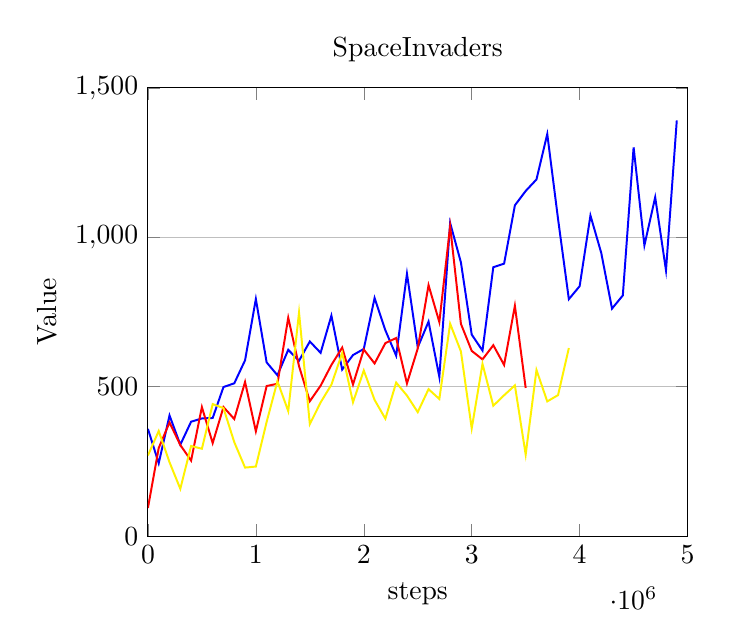
\begin{tikzpicture}

\begin{axis}[%
title=SpaceInvaders,
%width=10in,
%height=5in,
%at={(2.596in,2.358in)},
% scale only axis,
xmin=0,
xmax=5000000,
xlabel style={font=\color{white!15!black}},
xlabel={steps},
xlabel near ticks,
ymin=0,
ymax=1500,
ylabel style={font=\color{white!15!black}},
ylabel={Value},
ylabel near ticks,
ymajorgrids,
% %scale=0.5,
%scale=0.4,
axis background/.style={fill=white},
%legend style={legend cell align=left, align=left, draw=white!15!black}
]
\addplot [color=blue, line width = 0.25mm]
                table[row sep=crcr]{
                  0 359.0\\ 
100000 244.0\\ 
200000 404.0\\ 
300000 306.0\\ 
400000 383.0\\ 
500000 394.0\\ 
600000 395.5\\ 
700000 499.0\\ 
800000 511.5\\ 
900000 588.5\\ 
1000000 793.5\\ 
1100000 581.5\\ 
1200000 538.5\\ 
1300000 623.5\\ 
1400000 587.0\\ 
1500000 651.5\\ 
1600000 613.5\\ 
1700000 738.0\\ 
1800000 557.5\\ 
1900000 606.0\\ 
2000000 626.5\\ 
2100000 797.0\\ 
2200000 689.0\\ 
2300000 604.0\\ 
2400000 878.0\\ 
2500000 632.0\\ 
2600000 718.0\\ 
2700000 533.0\\ 
2800000 1048.0\\ 
2900000 916.0\\ 
3000000 674.5\\ 
3100000 621.0\\ 
3200000 900.0\\ 
3300000 912.0\\ 
3400000 1107.0\\ 
3500000 1155.0\\ 
3600000 1193.5\\ 
3700000 1345.5\\ 
3800000 1061.0\\ 
3900000 793.0\\ 
4000000 836.5\\ 
4100000 1073.0\\ 
4200000 948.0\\ 
4300000 761.5\\ 
4400000 805.5\\ 
4500000 1301.0\\ 
4600000 973.0\\ 
4700000 1134.0\\ 
4800000 889.5\\ 
4900000 1391.0\\ 
};
\addplot [color=red, line width = 0.25mm]
                table[row sep=crcr]{
                  0 94.5\\ 
100000 295.0\\ 
200000 380.5\\ 
300000 305.0\\ 
400000 253.0\\ 
500000 432.0\\ 
600000 311.5\\ 
700000 432.0\\ 
800000 392.0\\ 
900000 516.0\\ 
1000000 351.0\\ 
1100000 502.5\\ 
1200000 510.0\\ 
1300000 731.0\\ 
1400000 569.0\\ 
1500000 451.5\\ 
1600000 503.5\\ 
1700000 573.0\\ 
1800000 631.0\\ 
1900000 507.5\\ 
2000000 624.5\\ 
2100000 578.0\\ 
2200000 646.0\\ 
2300000 663.0\\ 
2400000 511.0\\ 
2500000 628.0\\ 
2600000 840.0\\ 
2700000 716.5\\ 
2800000 1037.0\\ 
2900000 710.5\\ 
3000000 620.0\\ 
3100000 591.5\\ 
3200000 639.0\\ 
3300000 573.0\\ 
3400000 771.0\\ 
3500000 496.0\\ 
};
\addplot [color=yellow, line width = 0.25mm]
                table[row sep=crcr]{
                  0 270.0\\ 
100000 352.0\\ 
200000 247.5\\ 
300000 158.5\\ 
400000 302.0\\ 
500000 292.5\\ 
600000 442.0\\ 
700000 428.5\\ 
800000 314.5\\ 
900000 229.5\\ 
1000000 233.0\\ 
1100000 382.5\\ 
1200000 518.5\\ 
1300000 418.5\\ 
1400000 748.5\\ 
1500000 375.0\\ 
1600000 447.5\\ 
1700000 507.0\\ 
1800000 613.0\\ 
1900000 448.0\\ 
2000000 554.5\\ 
2100000 456.0\\ 
2200000 393.0\\ 
2300000 514.0\\ 
2400000 470.5\\ 
2500000 415.0\\ 
2600000 492.0\\ 
2700000 459.0\\ 
2800000 711.0\\ 
2900000 618.0\\ 
3000000 360.5\\ 
3100000 576.5\\ 
3200000 436.5\\ 
3300000 471.5\\ 
3400000 504.5\\ 
3500000 273.0\\ 
3600000 556.0\\ 
3700000 451.0\\ 
3800000 472.0\\ 
3900000 629.5\\ 
};
\end{axis}
\end{tikzpicture}}}
  \\

  \ref{named}
  \caption{Effectiveness of parallel training. Overall the results are negative, some slightly
  and others strongly. Interestingly, using a pretrained encoder has a negative effect
in this case. We suspect that this is due to the fixation on a particular local minimum caused
by reconstruction loss. Importantly, the negative effect is present despite
regularization maintaining a fixed latent space over a relatively large number of epochs (5-10).
Results tend to be worse in games where MSE loss is less suitable and in games
with larger visual complexity.}
  \label{fig:parallel}
\end{figure}

Before continuing the discussion, the effectiveness of regularization needs to be discussed.
We present runs with both data augmentation and L2 regularization and
those without either in \ref{fig:reg-vs-no-reg}.

\begin{figure}[!t]
  \captionsetup[subfloat]{position=top,labelformat=empty}
  \centering

    \subfloat[]{  \resizebox{0.4\textwidth}{!}{
%\definecolor{blue}{RGB}{76,100,135}
%\definecolor{red}{RGB}{153,0,0}
%\definecolor{yellow}{RGB}{227,178,60}
%\definecolor{mycolor1}{rgb}{0.00000,0.44700,0.74100}%
%\definecolor{mycolor2}{rgb}{0.85000,0.32500,0.09800}%
%\definecolor{mycolor3}{rgb}{0.92900,0.69400,0.12500}%
%
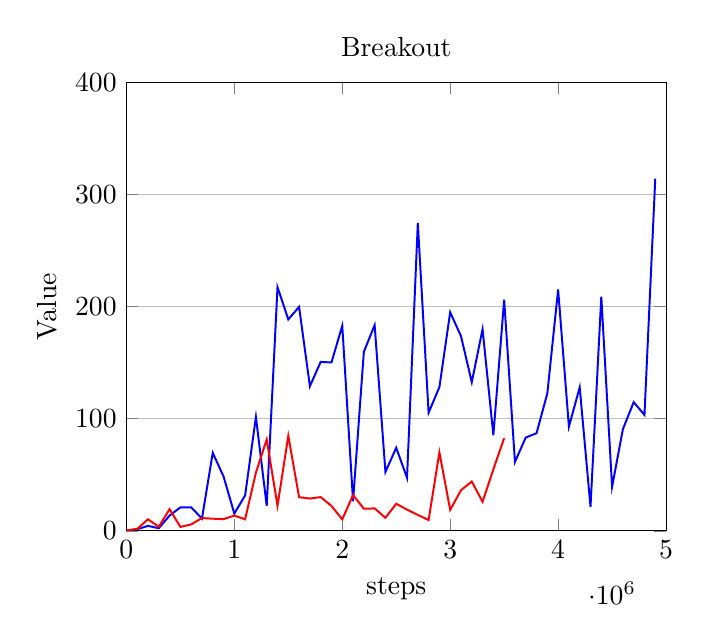
\begin{tikzpicture}

\begin{axis}[%
legend entries={rl-only-small-net,L2-reg,parallel-fs-50-no-aug}, 
legend columns=2,
title=Breakout,
legend to name=named,
legend style={legend cell align=left},
%%width=10in,
%%height=5in,
%%at={(2.596in,2.358in)},
% scale only axis,
xmin=0,
xmax=5000000,
xlabel style={font=\color{white!15!black}},
xlabel={steps},
xlabel near ticks,
ymin=0,
ymax=400,
ylabel style={font=\color{white!15!black}},
ylabel={Value},
ylabel near ticks,
ymajorgrids,
% %scale=0.5,
%%scale=0.4,
axis background/.style={fill=white},
%legend columns=2,
%legend=south outside
]
\addplot [color=blue, line width = 0.25mm]
                table[row sep=crcr]{
                  0 0.20000000298023224\\ 
100000 1.399999976158142\\ 
200000 4.400000095367432\\ 
300000 2.299999952316284\\ 
400000 13.600000381469727\\ 
500000 20.899999618530273\\ 
600000 21.0\\ 
700000 10.899999618530273\\ 
800000 69.5999984741211\\ 
900000 48.5\\ 
1000000 15.399999618530273\\ 
1100000 31.600000381469727\\ 
1200000 101.5999984741211\\ 
1300000 22.399999618530273\\ 
1400000 217.39999389648438\\ 
1500000 188.60000610351562\\ 
1600000 199.8000030517578\\ 
1700000 129.0\\ 
1800000 150.6999969482422\\ 
1900000 150.1999969482422\\ 
2000000 183.0\\ 
2100000 26.399999618530273\\ 
2200000 159.6999969482422\\ 
2300000 183.5\\ 
2400000 52.5\\ 
2500000 74.0999984741211\\ 
2600000 47.29999923706055\\ 
2700000 274.6000061035156\\ 
2800000 105.4000015258789\\ 
2900000 128.1999969482422\\ 
3000000 195.0\\ 
3100000 173.6999969482422\\ 
3200000 132.60000610351562\\ 
3300000 179.89999389648438\\ 
3400000 85.19999694824219\\ 
3500000 206.1999969482422\\ 
3600000 61.5\\ 
3700000 83.19999694824219\\ 
3800000 87.0999984741211\\ 
3900000 122.5999984741211\\ 
4000000 215.3000030517578\\ 
4100000 92.9000015258789\\ 
4200000 128.0\\ 
4300000 21.399999618530273\\ 
4400000 208.89999389648438\\ 
4500000 39.20000076293945\\ 
4600000 90.5999984741211\\ 
4700000 114.80000305175781\\ 
4800000 103.4000015258789\\ 
4900000 314.20001220703125\\ 
};
\addplot [color=red, line width = 0.25mm]
                table[row sep=crcr]{
                  0 0.4000000059604645\\ 
100000 1.7000000476837158\\ 
200000 10.300000190734863\\ 
300000 3.5999999046325684\\ 
400000 19.299999237060547\\ 
500000 3.5\\ 
600000 5.699999809265137\\ 
700000 11.399999618530273\\ 
800000 10.800000190734863\\ 
900000 10.399999618530273\\ 
1000000 13.600000381469727\\ 
1100000 10.300000190734863\\ 
1200000 51.900001525878906\\ 
1300000 81.5\\ 
1400000 22.299999237060547\\ 
1500000 84.69999694824219\\ 
1600000 30.0\\ 
1700000 28.799999237060547\\ 
1800000 30.100000381469727\\ 
1900000 22.200000762939453\\ 
2000000 10.199999809265137\\ 
2100000 31.899999618530273\\ 
2200000 19.700000762939453\\ 
2300000 20.0\\ 
2400000 11.600000381469727\\ 
2500000 24.200000762939453\\ 
2600000 18.899999618530273\\ 
2700000 14.199999809265137\\ 
2800000 9.600000381469727\\ 
2900000 70.0\\ 
3000000 18.700000762939453\\ 
3100000 36.20000076293945\\ 
3200000 44.0\\ 
3300000 25.899999618530273\\ 
3400000 54.900001525878906\\ 
3500000 82.69999694824219\\ 
};
\addplot [color=yellow, line width = 0.25mm]
                table[row sep=crcr]{
                  0 0.800000011920929\\ 
};
\end{axis}
\end{tikzpicture}}}
    \subfloat[]{  \resizebox{0.4\textwidth}{!}{
%\definecolor{blue}{RGB}{76,100,135}
%\definecolor{red}{RGB}{153,0,0}
%\definecolor{yellow}{RGB}{227,178,60}
%\definecolor{mycolor1}{rgb}{0.00000,0.44700,0.74100}%
%\definecolor{mycolor2}{rgb}{0.85000,0.32500,0.09800}%
%\definecolor{mycolor3}{rgb}{0.92900,0.69400,0.12500}%
%
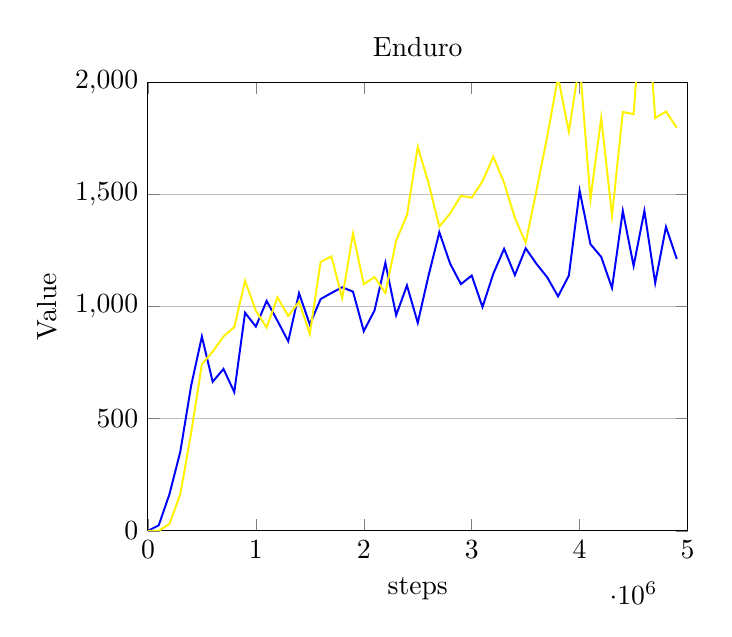
\begin{tikzpicture}

\begin{axis}[%
title=Enduro,
% %width=4.634in,
%%width=10in,
%%height=5in,
%at={(2.596in,2.358in)},
% scale only axis,
xmin=0,
xmax=5000000,
xlabel style={font=\color{white!15!black}},
xlabel={steps},
xlabel near ticks,
ymin=0,
ymax=2000,
ylabel style={font=\color{white!15!black}},
ylabel={Value},
ylabel near ticks,
ymajorgrids,
% %scale=0.5,
%scale=0.4,
axis background/.style={fill=white},
%legend style={legend cell align=left, align=left, draw=white!15!black}
]
\addplot [color=blue, line width = 0.25mm]
                table[row sep=crcr]{
                  0 0.0\\ 
100000 24.299999237060547\\ 
200000 164.3000030517578\\ 
300000 353.0\\ 
400000 646.4000244140625\\ 
500000 866.7000122070312\\ 
600000 664.7000122070312\\ 
700000 722.2000122070312\\ 
800000 618.9000244140625\\ 
900000 972.7999877929688\\ 
1000000 910.9000244140625\\ 
1100000 1025.699951171875\\ 
1200000 937.0\\ 
1300000 845.5999755859375\\ 
1400000 1059.9000244140625\\ 
1500000 920.2999877929688\\ 
1600000 1033.800048828125\\ 
1700000 1061.0\\ 
1800000 1086.5999755859375\\ 
1900000 1066.9000244140625\\ 
2000000 890.9000244140625\\ 
2100000 983.5\\ 
2200000 1195.300048828125\\ 
2300000 962.0\\ 
2400000 1094.800048828125\\ 
2500000 928.0\\ 
2600000 1138.5999755859375\\ 
2700000 1332.300048828125\\ 
2800000 1191.800048828125\\ 
2900000 1100.5999755859375\\ 
3000000 1138.800048828125\\ 
3100000 998.2999877929688\\ 
3200000 1146.800048828125\\ 
3300000 1258.0999755859375\\ 
3400000 1141.0\\ 
3500000 1260.300048828125\\ 
3600000 1190.800048828125\\ 
3700000 1130.5999755859375\\ 
3800000 1046.0999755859375\\ 
3900000 1138.4000244140625\\ 
4000000 1517.5\\ 
4100000 1278.9000244140625\\ 
4200000 1221.699951171875\\ 
4300000 1083.199951171875\\ 
4400000 1426.9000244140625\\ 
4500000 1181.5999755859375\\ 
4600000 1427.199951171875\\ 
4700000 1105.800048828125\\ 
4800000 1355.800048828125\\ 
4900000 1212.9000244140625\\ 
};
\addplot [color=red, line width = 0.25mm]
                table[row sep=crcr]{
                  0 0.0\\ 
};
\addplot [color=yellow, line width = 0.25mm]
                table[row sep=crcr]{
                  0 0.0\\ 
100000 0.0\\ 
200000 30.700000762939453\\ 
300000 163.6999969482422\\ 
400000 435.79998779296875\\ 
500000 743.2000122070312\\ 
600000 799.2000122070312\\ 
700000 867.0\\ 
800000 908.4000244140625\\ 
900000 1115.300048828125\\ 
1000000 981.4000244140625\\ 
1100000 906.9000244140625\\ 
1200000 1041.5999755859375\\ 
1300000 958.5999755859375\\ 
1400000 1021.9000244140625\\ 
1500000 877.7000122070312\\ 
1600000 1199.4000244140625\\ 
1700000 1224.0\\ 
1800000 1038.199951171875\\ 
1900000 1326.0999755859375\\ 
2000000 1100.0\\ 
2100000 1132.0999755859375\\ 
2200000 1060.9000244140625\\ 
2300000 1294.300048828125\\ 
2400000 1407.699951171875\\ 
2500000 1712.5\\ 
2600000 1551.5\\ 
2700000 1357.0\\ 
2800000 1415.800048828125\\ 
2900000 1494.5\\ 
3000000 1486.0\\ 
3100000 1559.699951171875\\ 
3200000 1668.5\\ 
3300000 1552.800048828125\\ 
3400000 1395.800048828125\\ 
3500000 1284.9000244140625\\ 
3600000 1518.0\\ 
3700000 1759.5999755859375\\ 
3800000 2024.9000244140625\\ 
3900000 1780.0999755859375\\ 
4000000 2090.5\\ 
4100000 1479.0999755859375\\ 
4200000 1841.699951171875\\ 
4300000 1405.5999755859375\\ 
4400000 1868.300048828125\\ 
4500000 1858.699951171875\\ 
4600000 2527.0\\ 
4700000 1841.0\\ 
4800000 1870.800048828125\\ 
4900000 1797.9000244140625\\ 
};
\end{axis}
\end{tikzpicture}}}\\
  \vspace{-1cm}
    \subfloat[]{  \resizebox{0.4\textwidth}{!}{
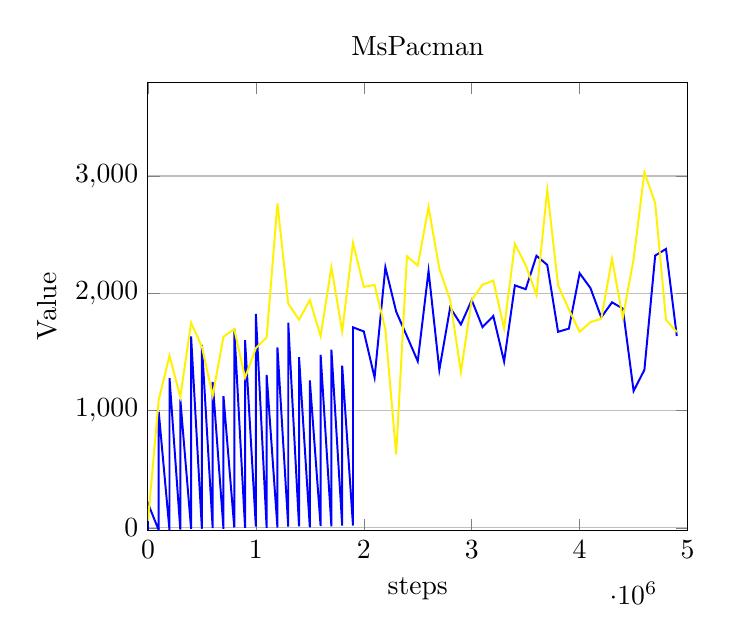
\begin{tikzpicture}

\begin{axis}[%
title=MsPacman,
% %width=4.634in,
%width=10in,
%height=5in,
%at={(2.596in,2.358in)},
% scale only axis,
xmin=0,
xmax=5000000,
xlabel style={font=\color{white!15!black}},
xlabel={steps},
xlabel near ticks,
ymin=-22,
ymax=3800,
ylabel style={font=\color{white!15!black}},
ylabel={Value},
ylabel near ticks,
ymajorgrids,
% %scale=0.5,
%scale=0.4,
axis background/.style={fill=white},
%legend style={legend cell align=left, align=left, draw=white!15!black}
]
\addplot [color=blue, line width = 0.25mm]
                table[row sep=crcr]{
                  0 -21.0\\ 
0 210.0\\ 
100000 -19.799999237060547\\ 
100000 990.0\\ 
200000 -20.700000762939453\\ 
200000 1277.0\\ 
300000 -15.0\\ 
300000 1096.0\\ 
400000 -7.0\\ 
400000 1632.0\\ 
500000 -6.900000095367432\\ 
500000 1561.0\\ 
600000 -1.899999976158142\\ 
600000 1245.0\\ 
700000 -7.599999904632568\\ 
700000 1123.0\\ 
800000 4.0\\ 
800000 1696.0\\ 
900000 1.5\\ 
900000 1600.0\\ 
1000000 11.300000190734863\\ 
1000000 1824.0\\ 
1100000 1.2000000476837158\\ 
1100000 1304.0\\ 
1200000 3.700000047683716\\ 
1200000 1538.0\\ 
1300000 11.5\\ 
1300000 1750.0\\ 
1400000 13.600000381469727\\ 
1400000 1456.0\\ 
1500000 5.699999809265137\\ 
1500000 1258.0\\ 
1600000 15.600000381469727\\ 
1600000 1476.0\\ 
1700000 13.5\\ 
1700000 1519.0\\ 
1800000 19.299999237060547\\ 
1800000 1383.0\\ 
1900000 20.799999237060547\\ 
1900000 1710.0\\ 
2000000 1675.0\\ 
2100000 1282.0\\ 
2200000 2222.0\\ 
2300000 1844.0\\ 
2400000 1634.0\\ 
2500000 1421.0\\ 
2600000 2191.0\\ 
2700000 1347.0\\ 
2800000 1878.0\\ 
2900000 1735.0\\ 
3000000 1942.0\\ 
3100000 1712.0\\ 
3200000 1806.0\\ 
3300000 1419.0\\ 
3400000 2068.0\\ 
3500000 2035.0\\ 
3600000 2320.0\\ 
3700000 2242.0\\ 
3800000 1672.0\\ 
3900000 1699.0\\ 
4000000 2171.0\\ 
4100000 2045.0\\ 
4200000 1795.0\\ 
4300000 1923.0\\ 
4400000 1870.0\\ 
4500000 1167.0\\ 
4600000 1348.0\\ 
4700000 2322.0\\ 
4800000 2378.0\\ 
4900000 1636.0\\ 
};
\addplot [color=red, line width = 0.25mm]
                table[row sep=crcr]{
                  0 0.0\\ 
};
\addplot [color=yellow, line width = 0.25mm]
                table[row sep=crcr]{
                  0 60.0\\ 
100000 1090.0\\ 
200000 1469.0\\ 
300000 1117.0\\ 
400000 1749.0\\ 
500000 1545.0\\ 
600000 1128.0\\ 
700000 1630.0\\ 
800000 1695.0\\ 
900000 1281.0\\ 
1000000 1532.0\\ 
1100000 1625.0\\ 
1200000 2767.0\\ 
1300000 1912.0\\ 
1400000 1775.0\\ 
1500000 1942.0\\ 
1600000 1636.0\\ 
1700000 2222.0\\ 
1800000 1676.0\\ 
1900000 2430.0\\ 
2000000 2055.0\\ 
2100000 2072.0\\ 
2200000 1693.0\\ 
2300000 625.0\\ 
2400000 2317.0\\ 
2500000 2236.0\\ 
2600000 2736.0\\ 
2700000 2209.0\\ 
2800000 1944.0\\ 
2900000 1329.0\\ 
3000000 1944.0\\ 
3100000 2074.0\\ 
3200000 2109.0\\ 
3300000 1701.0\\ 
3400000 2421.0\\ 
3500000 2240.0\\ 
3600000 1986.0\\ 
3700000 2883.0\\ 
3800000 2069.0\\ 
3900000 1863.0\\ 
4000000 1672.0\\ 
4100000 1754.0\\ 
4200000 1783.0\\ 
4300000 2293.0\\ 
4400000 1791.0\\ 
4500000 2293.0\\ 
4600000 3033.0\\ 
4700000 2768.0\\ 
4800000 1774.0\\ 
4900000 1670.0\\ 
};
\end{axis}
\end{tikzpicture}}}
    \subfloat[]{  \resizebox{0.4\textwidth}{!}{
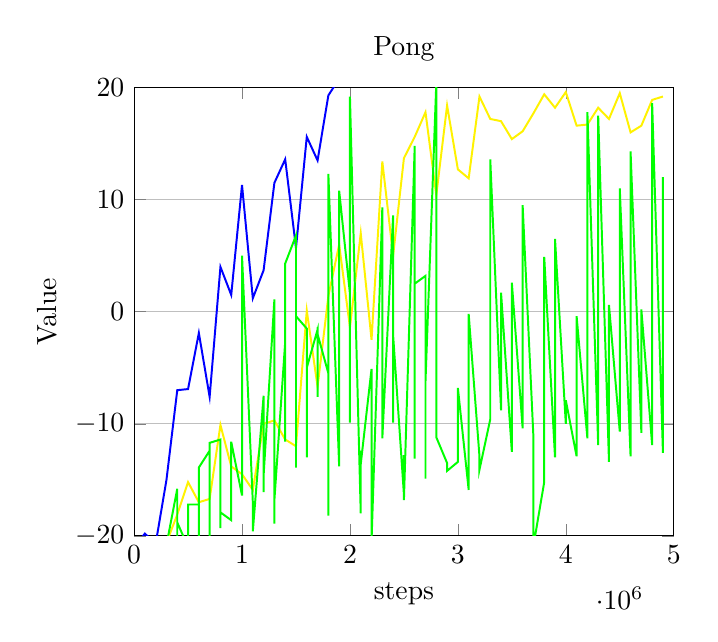
\begin{tikzpicture}

\begin{axis}[%
title=Pong,
% %width=4.634in,
%width=10in,
%height=5in,
%at={(2.596in,2.358in)},
% scale only axis,
xmin=0,
xmax=5000000,
xlabel style={font=\color{white!15!black}},
xlabel={steps},
xlabel near ticks,
ymin=-20,
ymax=20,
ylabel style={font=\color{white!15!black}},
ylabel={Value},
ylabel near ticks,
ymajorgrids,
% %scale=0.5,
%scale=0.4,
axis background/.style={fill=white},
%legend style={legend cell align=left, align=left, draw=white!15!black}
]
\addplot [color=blue, line width = 0.25mm]
                table[row sep=crcr]{
                  0 -21.0\\ 
100000 -19.799999237060547\\ 
200000 -20.700000762939453\\ 
300000 -15.0\\ 
400000 -7.0\\ 
500000 -6.900000095367432\\ 
600000 -1.899999976158142\\ 
700000 -7.599999904632568\\ 
800000 4.0\\ 
900000 1.5\\ 
1000000 11.300000190734863\\ 
1100000 1.2000000476837158\\ 
1200000 3.700000047683716\\ 
1300000 11.5\\ 
1400000 13.600000381469727\\ 
1500000 5.699999809265137\\ 
1600000 15.600000381469727\\ 
1700000 13.5\\ 
1800000 19.299999237060547\\ 
1900000 20.799999237060547\\ 
};
\addplot [color=red, line width = 0.25mm]
                table[row sep=crcr]{
                  0 0.0\\ 
};
\addplot [color=yellow, line width = 0.25mm]
                table[row sep=crcr]{
                  0 -21.0\\ 
0 -21.0\\ 
0 -21.0\\ 
100000 -21.0\\ 
200000 -20.299999237060547\\ 
300000 -20.600000381469727\\ 
400000 -18.100000381469727\\ 
500000 -15.199999809265137\\ 
600000 -17.0\\ 
700000 -16.700000762939453\\ 
800000 -10.100000381469727\\ 
900000 -13.800000190734863\\ 
1000000 -14.5\\ 
1100000 -15.899999618530273\\ 
1200000 -10.0\\ 
1300000 -9.699999809265137\\ 
1400000 -11.399999618530273\\ 
1500000 -12.0\\ 
1600000 0.10000000149011612\\ 
1700000 -6.699999809265137\\ 
1800000 1.399999976158142\\ 
1900000 6.0\\ 
2000000 -1.399999976158142\\ 
2100000 7.0\\ 
2200000 -2.5\\ 
2300000 13.399999618530273\\ 
2400000 5.0\\ 
2500000 13.699999809265137\\ 
2600000 15.600000381469727\\ 
2700000 17.799999237060547\\ 
2800000 10.399999618530273\\ 
2900000 18.399999618530273\\ 
3000000 12.699999809265137\\ 
3100000 11.899999618530273\\ 
3200000 19.200000762939453\\ 
3300000 17.200000762939453\\ 
3400000 17.0\\ 
3500000 15.399999618530273\\ 
3600000 16.100000381469727\\ 
3700000 17.700000762939453\\ 
3800000 19.399999618530273\\ 
3900000 18.200000762939453\\ 
4000000 19.600000381469727\\ 
4100000 16.600000381469727\\ 
4200000 16.700000762939453\\ 
4300000 18.200000762939453\\ 
4400000 17.200000762939453\\ 
4500000 19.5\\ 
4600000 16.0\\ 
4700000 16.600000381469727\\ 
4800000 18.899999618530273\\ 
4900000 19.200000762939453\\ 
};
\addplot [color=green, line width = 0.25mm]
                table[row sep=crcr]{
                  0 -21.0\\ 
0 -21.0\\ 
0 -21.0\\ 
0 -21.0\\ 
100000 -21.0\\ 
100000 -20.600000381469727\\ 
100000 -21.0\\ 
200000 -20.399999618530273\\ 
200000 -21.0\\ 
200000 -20.799999237060547\\ 
300000 -20.600000381469727\\ 
300000 -20.799999237060547\\ 
300000 -20.799999237060547\\ 
400000 -15.800000190734863\\ 
400000 -20.399999618530273\\ 
400000 -18.799999237060547\\ 
500000 -21.0\\ 
500000 -21.0\\ 
500000 -17.200000762939453\\ 
600000 -17.200000762939453\\ 
600000 -20.600000381469727\\ 
600000 -13.899999618530273\\ 
700000 -12.399999618530273\\ 
700000 -20.100000381469727\\ 
700000 -11.699999809265137\\ 
800000 -11.399999618530273\\ 
800000 -19.299999237060547\\ 
800000 -17.899999618530273\\ 
900000 -18.600000381469727\\ 
900000 -15.699999809265137\\ 
900000 -11.600000381469727\\ 
1000000 -16.399999618530273\\ 
1000000 -16.0\\ 
1000000 5.0\\ 
1100000 -17.0\\ 
1100000 -17.5\\ 
1100000 -19.600000381469727\\ 
1200000 -7.5\\ 
1200000 -16.100000381469727\\ 
1200000 -14.600000381469727\\ 
1300000 1.100000023841858\\ 
1300000 -18.899999618530273\\ 
1300000 -16.799999237060547\\ 
1400000 -2.700000047683716\\ 
1400000 -11.600000381469727\\ 
1400000 4.300000190734863\\ 
1500000 6.800000190734863\\ 
1500000 -13.899999618530273\\ 
1500000 -0.4000000059604645\\ 
1600000 -1.5\\ 
1600000 -13.0\\ 
1600000 -5.0\\ 
1700000 -1.600000023841858\\ 
1700000 -7.599999904632568\\ 
1700000 -2.0\\ 
1800000 -5.5\\ 
1800000 -18.200000762939453\\ 
1800000 12.300000190734863\\ 
1900000 -13.800000190734863\\ 
1900000 -10.0\\ 
1900000 10.800000190734863\\ 
2000000 1.600000023841858\\ 
2000000 -9.899999618530273\\ 
2000000 19.200000762939453\\ 
2100000 -18.0\\ 
2100000 -12.399999618530273\\ 
2100000 -13.600000381469727\\ 
2200000 -5.099999904632568\\ 
2200000 -13.899999618530273\\ 
2200000 -20.5\\ 
2300000 9.300000190734863\\ 
2300000 -8.199999809265137\\ 
2300000 -11.300000190734863\\ 
2400000 8.600000381469727\\ 
2400000 -9.899999618530273\\ 
2400000 -2.0999999046325684\\ 
2500000 -16.299999237060547\\ 
2500000 -12.800000190734863\\ 
2500000 -16.799999237060547\\ 
2600000 14.800000190734863\\ 
2600000 -13.100000381469727\\ 
2600000 2.5\\ 
2700000 3.200000047683716\\ 
2700000 -14.899999618530273\\ 
2700000 -6.199999809265137\\ 
2800000 20.399999618530273\\ 
2800000 -9.800000190734863\\ 
2800000 -11.199999809265137\\ 
2900000 -13.5\\ 
2900000 -14.199999809265137\\ 
3000000 -13.399999618530273\\ 
3000000 -6.800000190734863\\ 
3100000 -15.899999618530273\\ 
3100000 -0.20000000298023224\\ 
3200000 -12.899999618530273\\ 
3200000 -14.100000381469727\\ 
3300000 -9.600000381469727\\ 
3300000 13.600000381469727\\ 
3400000 -8.800000190734863\\ 
3400000 1.7000000476837158\\ 
3500000 -12.5\\ 
3500000 2.5999999046325684\\ 
3600000 -10.399999618530273\\ 
3600000 9.5\\ 
3700000 -11.199999809265137\\ 
3700000 -20.899999618530273\\ 
3800000 -15.199999809265137\\ 
3800000 4.900000095367432\\ 
3900000 -13.0\\ 
3900000 6.5\\ 
4000000 -10.0\\ 
4000000 -7.900000095367432\\ 
4100000 -12.899999618530273\\ 
4100000 -0.4000000059604645\\ 
4200000 -11.300000190734863\\ 
4200000 17.799999237060547\\ 
4300000 -11.899999618530273\\ 
4300000 17.5\\ 
4400000 -13.399999618530273\\ 
4400000 0.6000000238418579\\ 
4500000 -10.699999809265137\\ 
4500000 11.0\\ 
4600000 -12.899999618530273\\ 
4600000 14.300000190734863\\ 
4700000 -10.800000190734863\\ 
4700000 0.20000000298023224\\ 
4800000 -11.899999618530273\\ 
4800000 18.600000381469727\\ 
4900000 -12.600000381469727\\ 
4900000 12.0\\ 
};
\end{axis}
\end{tikzpicture}}}\\
  \vspace{-1cm}
    \subfloat[]{  \resizebox{0.4\textwidth}{!}{
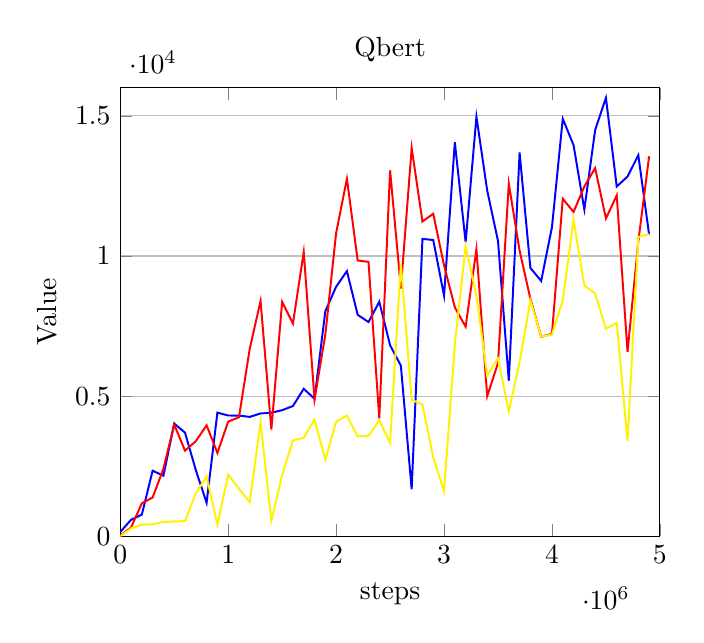
\begin{tikzpicture}

\begin{axis}[%
title=Qbert,
% %width=4.634in,
%width=10in,
%height=5in,
%at={(2.596in,2.358in)},
% scale only axis,
xmin=0,
xmax=5000000,
xlabel style={font=\color{white!15!black}},
xlabel={steps},
xlabel near ticks,
ymin=0,
ymax=16000,
ylabel style={font=\color{white!15!black}},
ylabel={Value},
ylabel near ticks,
ymajorgrids,
% %scale=0.5,
%scale=0.4,
axis background/.style={fill=white},
%legend style={legend cell align=left, align=left, draw=white!15!black}
]
\addplot [color=blue, line width = 0.25mm]
                table[row sep=crcr]{
                  0 150.0\\ 
100000 585.0\\ 
200000 772.5\\ 
300000 2337.5\\ 
400000 2157.5\\ 
500000 4022.5\\ 
600000 3695.0\\ 
700000 2362.5\\ 
800000 1192.5\\ 
900000 4410.0\\ 
1000000 4307.5\\ 
1100000 4305.0\\ 
1200000 4257.5\\ 
1300000 4380.0\\ 
1400000 4407.5\\ 
1500000 4497.5\\ 
1600000 4645.0\\ 
1700000 5260.0\\ 
1800000 4905.0\\ 
1900000 8030.0\\ 
2000000 8902.5\\ 
2100000 9460.0\\ 
2200000 7900.0\\ 
2300000 7642.5\\ 
2400000 8367.5\\ 
2500000 6815.0\\ 
2600000 6085.0\\ 
2700000 1677.5\\ 
2800000 10610.0\\ 
2900000 10570.0\\ 
3000000 8585.0\\ 
3100000 14057.5\\ 
3200000 10490.0\\ 
3300000 14970.0\\ 
3400000 12332.5\\ 
3500000 10537.5\\ 
3600000 5550.0\\ 
3700000 13692.5\\ 
3800000 9572.5\\ 
3900000 9110.0\\ 
4000000 11030.0\\ 
4100000 14897.5\\ 
4200000 13955.0\\ 
4300000 11660.0\\ 
4400000 14495.0\\ 
4500000 15645.0\\ 
4600000 12480.0\\ 
4700000 12835.0\\ 
4800000 13597.5\\ 
4900000 10762.5\\ 
};
\addplot [color=red, line width = 0.25mm]
                table[row sep=crcr]{
                  0 22.5\\ 
100000 310.0\\ 
200000 1172.5\\ 
300000 1382.5\\ 
400000 2410.0\\ 
500000 3982.5\\ 
600000 3052.5\\ 
700000 3390.0\\ 
800000 3957.5\\ 
900000 2970.0\\ 
1000000 4090.0\\ 
1100000 4245.0\\ 
1200000 6697.5\\ 
1300000 8395.0\\ 
1400000 3807.5\\ 
1500000 8360.0\\ 
1600000 7590.0\\ 
1700000 10142.5\\ 
1800000 4877.5\\ 
1900000 7190.0\\ 
2000000 10817.5\\ 
2100000 12755.0\\ 
2200000 9840.0\\ 
2300000 9790.0\\ 
2400000 4202.5\\ 
2500000 13057.5\\ 
2600000 8842.5\\ 
2700000 13852.5\\ 
2800000 11230.0\\ 
2900000 11507.5\\ 
3000000 9665.0\\ 
3100000 8167.5\\ 
3200000 7475.0\\ 
3300000 10242.5\\ 
3400000 4997.5\\ 
3500000 6180.0\\ 
3600000 12582.5\\ 
3700000 10190.0\\ 
3800000 8475.0\\ 
3900000 7115.0\\ 
4000000 7222.5\\ 
4100000 12042.5\\ 
4200000 11572.5\\ 
4300000 12480.0\\ 
4400000 13137.5\\ 
4500000 11337.5\\ 
4600000 12165.0\\ 
4700000 6580.0\\ 
4800000 10517.5\\ 
4900000 13560.0\\ 
};
\addplot [color=yellow, line width = 0.25mm]
                table[row sep=crcr]{
                  0 0.0\\ 
100000 280.0\\ 
200000 415.0\\ 
300000 425.0\\ 
400000 507.5\\ 
500000 525.0\\ 
600000 537.5\\ 
700000 1525.0\\ 
800000 2137.5\\ 
900000 407.5\\ 
1000000 2195.0\\ 
1100000 1690.0\\ 
1200000 1215.0\\ 
1300000 4077.5\\ 
1400000 550.0\\ 
1500000 2185.0\\ 
1600000 3417.5\\ 
1700000 3512.5\\ 
1800000 4165.0\\ 
1900000 2730.0\\ 
2000000 4090.0\\ 
2100000 4305.0\\ 
2200000 3557.5\\ 
2300000 3585.0\\ 
2400000 4137.5\\ 
2500000 3335.0\\ 
2600000 9722.5\\ 
2700000 4865.0\\ 
2800000 4700.0\\ 
2900000 2812.5\\ 
3000000 1605.0\\ 
3100000 6847.5\\ 
3200000 10342.5\\ 
3300000 8590.0\\ 
3400000 5732.5\\ 
3500000 6345.0\\ 
3600000 4447.5\\ 
3700000 6217.5\\ 
3800000 8415.0\\ 
3900000 7120.0\\ 
4000000 7195.0\\ 
4100000 8415.0\\ 
4200000 11307.5\\ 
4300000 8942.5\\ 
4400000 8662.5\\ 
4500000 7402.5\\ 
4600000 7612.5\\ 
4700000 3395.0\\ 
4800000 10680.0\\ 
4900000 10780.0\\ 
};
\end{axis}
\end{tikzpicture}}}
    \subfloat[]{  \resizebox{0.4\textwidth}{!}{
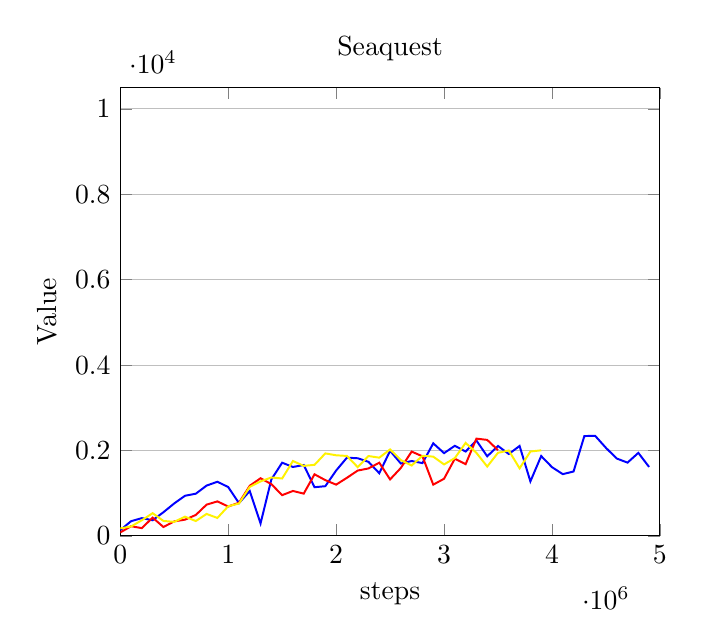
\begin{tikzpicture}

\begin{axis}[%
title=Seaquest,
% %width=4.634in,
%width=10in,
%height=5in,
%at={(2.596in,2.358in)},
% scale only axis,
xmin=0,
xmax=5000000,
xlabel style={font=\color{white!15!black}},
xlabel={steps},
xlabel near ticks,
ymin=0,
ymax=10500,
ylabel style={font=\color{white!15!black}},
ylabel={Value},
ylabel near ticks,
ymajorgrids,
% %scale=0.5,
%scale=0.4,
axis background/.style={fill=white},
%legend style={legend cell align=left, align=left, draw=white!15!black}
]
\addplot [color=blue, line width = 0.25mm]
                table[row sep=crcr]{
                  0 134.0\\ 
100000 344.0\\ 
200000 416.0\\ 
300000 366.0\\ 
400000 554.0\\ 
500000 760.0\\ 
600000 940.0\\ 
700000 988.0\\ 
800000 1178.0\\ 
900000 1268.0\\ 
1000000 1144.0\\ 
1100000 768.0\\ 
1200000 1052.0\\ 
1300000 292.0\\ 
1400000 1322.0\\ 
1500000 1714.0\\ 
1600000 1614.0\\ 
1700000 1660.0\\ 
1800000 1140.0\\ 
1900000 1164.0\\ 
2000000 1530.0\\ 
2100000 1832.0\\ 
2200000 1818.0\\ 
2300000 1734.0\\ 
2400000 1468.0\\ 
2500000 1992.0\\ 
2600000 1694.0\\ 
2700000 1754.0\\ 
2800000 1704.0\\ 
2900000 2168.0\\ 
3000000 1938.0\\ 
3100000 2110.0\\ 
3200000 1976.0\\ 
3300000 2234.0\\ 
3400000 1864.0\\ 
3500000 2106.0\\ 
3600000 1918.0\\ 
3700000 2106.0\\ 
3800000 1276.0\\ 
3900000 1870.0\\ 
4000000 1610.0\\ 
4100000 1446.0\\ 
4200000 1508.0\\ 
4300000 2338.0\\ 
4400000 2344.0\\ 
4500000 2062.0\\ 
4600000 1812.0\\ 
4700000 1716.0\\ 
4800000 1944.0\\ 
4900000 1614.0\\ 
};
\addplot [color=red, line width = 0.25mm]
                table[row sep=crcr]{
                  0 80.0\\ 
100000 226.0\\ 
200000 182.0\\ 
300000 428.0\\ 
400000 208.0\\ 
500000 340.0\\ 
600000 380.0\\ 
700000 490.0\\ 
800000 732.0\\ 
900000 808.0\\ 
1000000 688.0\\ 
1100000 776.0\\ 
1200000 1174.0\\ 
1300000 1350.0\\ 
1400000 1212.0\\ 
1500000 954.0\\ 
1600000 1052.0\\ 
1700000 990.0\\ 
1800000 1442.0\\ 
1900000 1306.0\\ 
2000000 1200.0\\ 
2100000 1360.0\\ 
2200000 1530.0\\ 
2300000 1580.0\\ 
2400000 1714.0\\ 
2500000 1322.0\\ 
2600000 1592.0\\ 
2700000 1974.0\\ 
2800000 1864.0\\ 
2900000 1200.0\\ 
3000000 1338.0\\ 
3100000 1808.0\\ 
3200000 1680.0\\ 
3300000 2278.0\\ 
3400000 2248.0\\ 
3500000 2008.0\\ 
};
\addplot [color=yellow, line width = 0.25mm]
                table[row sep=crcr]{
                  0 176.0\\ 
100000 220.0\\ 
200000 366.0\\ 
300000 532.0\\ 
400000 350.0\\ 
500000 328.0\\ 
600000 450.0\\ 
700000 348.0\\ 
800000 514.0\\ 
900000 420.0\\ 
1000000 694.0\\ 
1100000 758.0\\ 
1200000 1148.0\\ 
1300000 1276.0\\ 
1400000 1368.0\\ 
1500000 1344.0\\ 
1600000 1754.0\\ 
1700000 1640.0\\ 
1800000 1664.0\\ 
1900000 1932.0\\ 
2000000 1888.0\\ 
2100000 1872.0\\ 
2200000 1610.0\\ 
2300000 1870.0\\ 
2400000 1832.0\\ 
2500000 2024.0\\ 
2600000 1774.0\\ 
2700000 1648.0\\ 
2800000 1876.0\\ 
2900000 1856.0\\ 
3000000 1674.0\\ 
3100000 1822.0\\ 
3200000 2178.0\\ 
3300000 1944.0\\ 
3400000 1624.0\\ 
3500000 1946.0\\ 
3600000 2000.0\\ 
3700000 1582.0\\ 
3800000 1976.0\\ 
3900000 2004.0\\ 
};
\end{axis}
\end{tikzpicture}}}\\
  \vspace{-1cm}
    \subfloat[]{  \resizebox{0.4\textwidth}{!}{
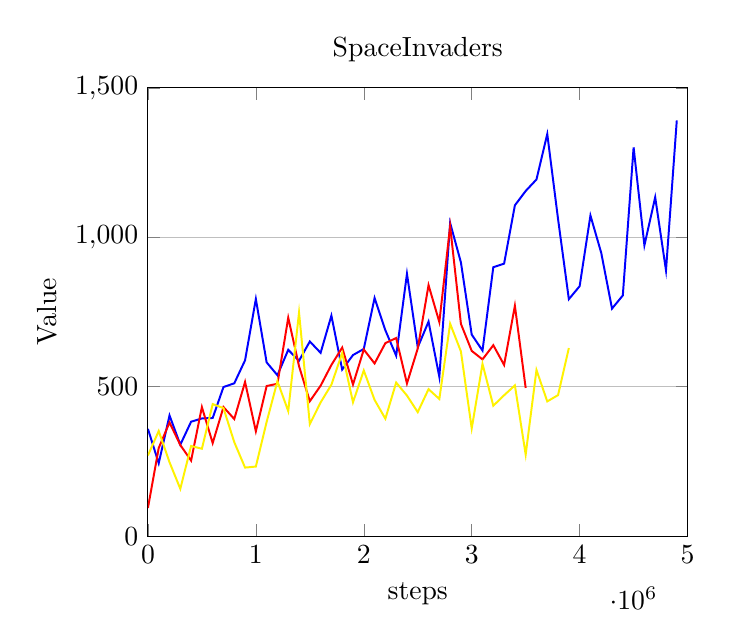
\begin{tikzpicture}

\begin{axis}[%
title=SpaceInvaders,
%width=10in,
%height=5in,
%at={(2.596in,2.358in)},
% scale only axis,
xmin=0,
xmax=5000000,
xlabel style={font=\color{white!15!black}},
xlabel={steps},
xlabel near ticks,
ymin=0,
ymax=1500,
ylabel style={font=\color{white!15!black}},
ylabel={Value},
ylabel near ticks,
ymajorgrids,
% %scale=0.5,
%scale=0.4,
axis background/.style={fill=white},
%legend style={legend cell align=left, align=left, draw=white!15!black}
]
\addplot [color=blue, line width = 0.25mm]
                table[row sep=crcr]{
                  0 359.0\\ 
100000 244.0\\ 
200000 404.0\\ 
300000 306.0\\ 
400000 383.0\\ 
500000 394.0\\ 
600000 395.5\\ 
700000 499.0\\ 
800000 511.5\\ 
900000 588.5\\ 
1000000 793.5\\ 
1100000 581.5\\ 
1200000 538.5\\ 
1300000 623.5\\ 
1400000 587.0\\ 
1500000 651.5\\ 
1600000 613.5\\ 
1700000 738.0\\ 
1800000 557.5\\ 
1900000 606.0\\ 
2000000 626.5\\ 
2100000 797.0\\ 
2200000 689.0\\ 
2300000 604.0\\ 
2400000 878.0\\ 
2500000 632.0\\ 
2600000 718.0\\ 
2700000 533.0\\ 
2800000 1048.0\\ 
2900000 916.0\\ 
3000000 674.5\\ 
3100000 621.0\\ 
3200000 900.0\\ 
3300000 912.0\\ 
3400000 1107.0\\ 
3500000 1155.0\\ 
3600000 1193.5\\ 
3700000 1345.5\\ 
3800000 1061.0\\ 
3900000 793.0\\ 
4000000 836.5\\ 
4100000 1073.0\\ 
4200000 948.0\\ 
4300000 761.5\\ 
4400000 805.5\\ 
4500000 1301.0\\ 
4600000 973.0\\ 
4700000 1134.0\\ 
4800000 889.5\\ 
4900000 1391.0\\ 
};
\addplot [color=red, line width = 0.25mm]
                table[row sep=crcr]{
                  0 94.5\\ 
100000 295.0\\ 
200000 380.5\\ 
300000 305.0\\ 
400000 253.0\\ 
500000 432.0\\ 
600000 311.5\\ 
700000 432.0\\ 
800000 392.0\\ 
900000 516.0\\ 
1000000 351.0\\ 
1100000 502.5\\ 
1200000 510.0\\ 
1300000 731.0\\ 
1400000 569.0\\ 
1500000 451.5\\ 
1600000 503.5\\ 
1700000 573.0\\ 
1800000 631.0\\ 
1900000 507.5\\ 
2000000 624.5\\ 
2100000 578.0\\ 
2200000 646.0\\ 
2300000 663.0\\ 
2400000 511.0\\ 
2500000 628.0\\ 
2600000 840.0\\ 
2700000 716.5\\ 
2800000 1037.0\\ 
2900000 710.5\\ 
3000000 620.0\\ 
3100000 591.5\\ 
3200000 639.0\\ 
3300000 573.0\\ 
3400000 771.0\\ 
3500000 496.0\\ 
};
\addplot [color=yellow, line width = 0.25mm]
                table[row sep=crcr]{
                  0 270.0\\ 
100000 352.0\\ 
200000 247.5\\ 
300000 158.5\\ 
400000 302.0\\ 
500000 292.5\\ 
600000 442.0\\ 
700000 428.5\\ 
800000 314.5\\ 
900000 229.5\\ 
1000000 233.0\\ 
1100000 382.5\\ 
1200000 518.5\\ 
1300000 418.5\\ 
1400000 748.5\\ 
1500000 375.0\\ 
1600000 447.5\\ 
1700000 507.0\\ 
1800000 613.0\\ 
1900000 448.0\\ 
2000000 554.5\\ 
2100000 456.0\\ 
2200000 393.0\\ 
2300000 514.0\\ 
2400000 470.5\\ 
2500000 415.0\\ 
2600000 492.0\\ 
2700000 459.0\\ 
2800000 711.0\\ 
2900000 618.0\\ 
3000000 360.5\\ 
3100000 576.5\\ 
3200000 436.5\\ 
3300000 471.5\\ 
3400000 504.5\\ 
3500000 273.0\\ 
3600000 556.0\\ 
3700000 451.0\\ 
3800000 472.0\\ 
3900000 629.5\\ 
};
\end{axis}
\end{tikzpicture}}}
  \\

  \ref{named}
  \caption{caption text 23}
  \label{fig:reg-vs-no-reg}
\end{figure}











\chapter{Discussion}
\label{ch-discussion}
